\documentclass[defaultstyle,10pt,master,Helvetica]{01.thesis}
%Use 01.thesis_pt instead for PT version 
%Dummy text if written by default in English. Just changed to whatever you need.
% Helvetica is a similar font to Arial, with small differences.

%% Packages
\typeout{}
\typeout{--------------------------------------------------------------}
\typeout{ +---+ Thesis Template                            }
\typeout{ +---+      Version 2.0, August 2011                         }
\typeout{ +---+  for Instituto Superior Tecnico (IST),                 }
\typeout{ +---+  Universidade Técnica de Lisboa                         }
\typeout{ * Using Thesis Style from Pedro Tomás                                }
\typeout{ * Created to write Dissertations                             }
\typeout{ * Conforms with IST Master Degree format and with most important packages setup        }
\typeout{ * Should conform with IST PhD Degree format (not verified)   }
\typeout{                                                              }
\typeout{ AUTHOR: Miguel Amador and João Marques                                          }
\typeout{                                                              }
\typeout{Important: Use all files in the archive, since this is based in all them. Modify dummy files at wish.                                                              }
\typeout{--------------------------------------------------------------}
\typeout{}

% Defines an additional alphabet... not required in most cases
% ------------------------------------------------------------
% \DeclareMathAlphabet{\mathpzc}{OT1}{pzc}{m}{it}

% PACKAGE babel:
% ---------------
% The 'babel' package may correct some hyphenisation issues of latex. 
% However in most situations it is not required.
\usepackage[english,portuguese]{babel}


% PACKAGE fontenc:
% -----------------
% chooses T1-fonts and allows correct automatic hyphenation.
%\usepackage[T1]{fontenc}
%\usepackage[latin1]{inputenc}
\usepackage[utf8]{inputenc}
%\usepackage{lmodern}

% Package ulem.
\usepackage{ulem} % Allows the use of other text emphatizer commands
\normalem %defines \emph{} to italic, instead of underline. 
\raggedbottom %declaration makes all pages the height of the text on that page. No extra vertical space is added. The \flushbottom declaration makes all text pages the same height, adding extra vertical space when necessary to fill out the page.

% PACKAGE date time:
% -----------------
% Lets you alter the format of the date that \today returns.
\usepackage{datetime}
\newdateformat{todaythesis}{%
\monthname[\THEMONTH]  \THEYEAR}

% PACKAGE latexsym:
% -----------------
% Defines additional latex symbols. May be required for thesis with many math symbols.
\usepackage{latexsym}

% PACKAGE amsmath, amsthm, amssymb, amsfonts:
% -------------------------------------------
% This package is typically required. Among many other things it adds the possibility
% to put symbols in bold by using \boldsymbol (not \mathbf); defines additional 
% fonts and symbols; adds the \eqref command for citing equations. I prefer the style
% "(x.xx)" for referering to an equation than to use "equation x.xx".
\usepackage{amsmath, amsthm, amssymb, amsfonts, amsbsy}

% PACKAGE multirow, colortbl, longtable:
% ---------------------------------------
% These packages are most usefull for advanced tables. The first allows to join rows 
% throuhg the command \multirow which works similarly with the command \multicolumn
% The second package allows to color the table (both foreground and background)
% The third package is only required when tables extend beyond the length of one page;
% with compatibilities with the tabular environment. The last allow the definitions of landscape pages, allowing the use of a different orientation for wider graphics or tables. See package documentation to see the implementation.
\usepackage{multirow}
\usepackage{colortbl}
\usepackage{supertabular}
\usepackage{pdflscape}
% \usepackage{longtable}

% PACKAGE graphics, epsfig, subfigure, caption:
% ---------------------------------------------
% Packages for figures... well you will certainly need these packages, with the exception
% of the 'caption' package. This only allows to define extra caption options.
% Notice that subfigure allows to place figures within figures with its own caption. It
% should be avoided to create an eps file with subfigures. That will mean that you won't be 
% able to reference those subfigures. Instead create an EPS file (the only graphics format supported
% by latex) for each of the subfigures and then use the command \subfigure (see below).
\usepackage{graphics}
\usepackage{graphicx}
\usepackage{epsfig}
\usepackage[hang,small,bf]{subfigure}
%\usepackage[footnotesize,bf,center]{caption}
\usepackage{dcolumn}
\usepackage{bm}
\usepackage{booktabs}
\usepackage{rotating}
\usepackage{multirow}

\usepackage[font=small,labelfont=bf,textfont=normalfont]{caption}

% PACKAGE algorithmic, algorithm
% ------------------------------
% These packages are required if you need to describe an algorithm.
% \usepackage{algorithmic}
% \usepackage[chapter]{algorithm}

% PACKAGE natbib/cite
% -------------------
% The two packages are not compatible, and you should use one of the two. Notice however that the
% IEEE BiBTeX stylesheet is imcompatible with the natbib package. If using the IEEE format, use the 
% cite package instead
%\usepackage[square,numbers,sort&compress]{natbib}
\usepackage{cite}

% PACKAGE acronyum
% -----------------
% This package is most useful for acronyms. The package guarantees that all acronyms definitions are 
% given at the first usage. IMPORTANT: do not use acronyms in titles/captions; otherwise the definition 
% will appear on the table of contents.
\usepackage{acronym}
\usepackage[titletoc,title,header]{appendix}
\usepackage[noauto]{chappg}

% PACKAGE extra_functions VER COMO DEVE SER
% -----------------
% My Personal package: defines the following commands:
% \fancychapter{chaptername) -> Prints a fancier chapter (you can also use the fancychapter package for this)
% \hline{width} -> use for a replacement of the \hline command
% \Mark1, \Mark2, \Mark3, ...
\usepackage{00.extra_functions}


% PACKAGE hyperref
% -----------------
% Set links for references and citations in document
% Some MiKTeX distributions have faulty PDF creators in which case this package will not work correctly
% Long live Linux :D
\usepackage[plainpages=false]{hyperref}
\hypersetup{
             colorlinks=false,
             citecolor=red,
             breaklinks=true,
             bookmarksnumbered=true,
             bookmarksopen=true,
             pdftitle={Thesis Title},
             pdfauthor={Author Name},
             pdfsubject={Master Thesis in Biomedical Engineering},
             pdfcreator={Document Creator Name},
             pdfkeywords={Template, Latex, Thesis}}
\usepackage{float}
%\usepackage[final]{00.listofsymbols}
\usepackage{00.symlist}

% Set paragraph counter to alphanumeric mode
\renewcommand{\theparagraph}{\Alph{paragraph}~--}

\newcommand{\figref}[1]{Figure \ref{#1}}
\newcommand{\equationref}[1]{Equation (\ref{#1})}
\newcommand{\tableref}[1]{Table (\ref{#1})}

\newcommand{\textreg}{$\textsuperscript{\textregistered}$}

%% Page formatting
\hoffset 0in
\voffset 0in

%Alternative set of page geometry
%\oddsidemargin 0.71cm
%\evensidemargin 0.04cm
%\marginparsep 0in
%\topmargin -0.25cm
%\textwidth 15cm
%\textheight 23.5cm

\usepackage[top=2.5cm, bottom=2.5cm, inner=2.9cm, outer=2.5cm]{geometry}

\usepackage{fancyhdr}
\pagestyle{fancy}
\renewcommand{\chaptermark}[1]{\markboth{\thechapter.\ #1}{}}
\renewcommand{\sectionmark}[1]{\markright{\thesection\ #1}}
\fancyhf{} 
%\fancyhead[LE]{\bfseries\nouppercase{\leftmark}}
%\fancyhead[RO]{\bfseries\nouppercase{\rightmark}}
\fancyfoot[LE,RO]{\bfseries\small\thepage}
\renewcommand{\headrulewidth}{0.0pt}
\renewcommand{\footrulewidth}{0.0pt}
\addtolength{\headheight}{2pt} % make space for the rule
\fancypagestyle{plain}{% Used in Chapter titles
   \fancyhead{} % get rid of headers
   \renewcommand{\headrulewidth}{0pt} % and the line
   \renewcommand{\footrulewidth}{0pt}
   \fancyfoot[LE,RO]{\bfseries\small\thepage}
}

\fancypagestyle{begin}{%
   \fancyhead{}
   \renewcommand{\headrulewidth}{0pt}
   \renewcommand{\footrulewidth}{0pt}
   \fancyfoot[LE,RO]{\bfseries\small\thepage}
}
\fancypagestyle{document}{%
	\fancyhf{} 
	\fancyhead[LE]{\bfseries\nouppercase{\leftmark}}
	\fancyhead[RO]{\bfseries\nouppercase{\rightmark}}
	\fancyfoot[LE,RO]{\bfseries\small\thepage}
	%\renewcommand{\headrulewidth}{0pt}
	%\renewcommand{\footrulewidth}{0pt}
	\addtolength{\headheight}{2pt} % make space for the rule
}
\fancypagestyle{documentsimple}{%
	\fancyhf{}
	\fancyfoot[LE,RO]{\bfseries\small\thepage}
	%\renewcommand{\headrulewidth}{0pt}
	%\renewcommand{\footrulewidth}{0pt}
	\addtolength{\headheight}{2pt} % make space for the rule
}
\setcounter{secnumdepth} {5}
\setcounter{tocdepth} {5}
\renewcommand{\thesubsubsection}{\thesubsection.\Alph{subsubsection}}

\renewcommand{\subfigtopskip}{0.3 cm}
\renewcommand{\subfigbottomskip}{0.2 cm}
\renewcommand{\subfigcapskip}{0.3 cm}
\renewcommand{\subfigcapmargin}{0.2 cm}

\graphicspath{{Figures/}}



%-----------------------------------------------------------
%-----------------------------------------------------------
\begin{document}
%% Use Main document Language
\selectlanguage{english}
%% ------
\pagestyle{begin}
\setcounter{page}{1} \pagenumbering{Alph}

% Add PDF bookmark 
\pdfbookmark[0]{Title}{Title}

\thispagestyle{empty}
\begin{flushleft} ~\\ \vspace{-12mm} \hspace{-12mm}  \includegraphics[width=50mm]{Cover/istnewlogo} 
\vspace{10mm}
%\\ \vspace{50mm} % gráficos
\\ \begin{center} \includegraphics[height=30mm]{Cover/dummy-pic.pdf}  \end{center} % gráficos
 \vspace{5mm}
\centering
\LARGE \textbf{A deep learning assessment of spike detection \\ with multi-electrode arrays}
\\ \vspace{10mm}
%\Large Subtitle
%\\ \vspace{15mm}
\Large \textbf{Pedro Corrêa Pereira Vasco de Lacerda} \\
\vspace{12mm}
\large Thesis to obtain the Master of Science Degree in
\\ \vspace{2mm}
\LARGE \textbf{Physics Engineering}
\\ \vspace{10mm}
\large Supervisor: Dr. Adam Raymond Kampff \\
\large Supervisor: Prof. Rui Manuel Agostinho Dilão
\\ \vspace{15mm}
\Large \textbf{Examination Committee}
\\ \vspace{5mm}
\large Chairperson:	Prof. A \\
\large Supervisor: Prof. Rui Manuel Agostinho Dilão \\
\large Members of the Committee: Prof. B \\
Prof. C
 
\vspace{15mm}

%\Large \textbf{\todaythesis\today} \\
\Large \textbf{April 2016} \\
\let\thepage\relax
\end{flushleft}
\pagebreak


\clearpage
% Since I am using double sided pages, the second page should be white.
% Remember that when delivering the dissertation, IST requires for the cover to appear twice.

\thispagestyle{empty}
\cleardoublepage

\setcounter{page}{1} \pagenumbering{roman}

\baselineskip 18pt % line spacing: -12pt for single spacing
                   %               -18pt for 1 1/2 spacing
                   %               -24pt for double spacingnts}
 
\pdfbookmark{Acknowledgments}{Acknowledgments}
\begin{acknowledgments} 
I would like to thank both my supervisors Dr. Adam R. Kampff and Prof. Rui Dilão for their guidance through out this project, as well as, to the Intelligent Systems laboratory in the Champalimaud Foundation for their inconditional help. I would like to thank my friends and family whose support was essential for me to accomplished this work.
\end{acknowledgments}
\clearpage
\thispagestyle{empty}
\cleardoublepage

\selectlanguage{english}
\begin{abstract}

To understand how the brain produces the diversity of behaviours observed in animals it is important to have quantitative methods to measure neural activity, particularly at the population level. Recent developments in integrated circuit design and microfabrication have made possible the production of large and dense multi-electrode arrays with hundreds of electrodes. However, computational methods to analyse the data recorded by these new generation probes did not keep up with the technological evolution. In Neto et al. (2016), a dataset from simultaneous in-vivo recordings of 128-channel dense extracellular silicon probe and a juxtacellular probe was first presented. In this work is reported the application of methods for deep learning to perform detection of Extracellular Action Potentials from this "ground-truth" data. Different models are tested and applied to several recordings in the dataset. The results are compared with a recent method from Rossant et al. (2016) called SpikeDetekt.

\end{abstract}

\begin{keywords}
Multi-electrode arrays, Extracellular Neurophysiology, Spike Detection, Deep Learning
\end{keywords}
\clearpage
\thispagestyle{empty}
\cleardoublepage

\selectlanguage{portuguese}
\begin{resumo}
Para compreender como os neurónios no cérebro produz a diversidade de comportamentos observados, é importante ter à nossa disposição métodos quantitativos e objectivos para medir a actividade neuronal, em particular ao nível das populações neuronais. Desenvolvimentos no design de circuito integrados e em microfabrição permitiu a produção de sondas de muito eléctrodos densas e de grandes dimensões com centenas de eléctrodos. No entanto, os métodos computationais para analisar os dados recolhidos com estas sondas de nova geração não acompanharam a evolução da tecnologia. Segundo Neto et al. (2016), os autores adquiriram dados simultâneos de sondas de vidro com 128 canais e uma pipeta juxtacelular. Neste documento está relatada a aplicação de métodos de aprendizagem usando redes neuronais artificiais profundas com o objectivo de fazer detecção de Potenciais de Acção Extracelulares nos acima mencionados. Foram testadas várias arquitecturas e configurações e aplicou-se a rede a diversos dados do conjunto. Os resultados são comparados com os dados obtido com o SpikeDetekt, método de detecção de Potenciais de Acção proposto por Rossant et al. (2016)
\end{resumo}

\begin{palavraschave}
Sondas de muitos eléctrodos, Neurofisiologia Extracelular, Detecção de potenciais de acção extracelulares, métodos de aprendizagem automática profunda
\end{palavraschave}
\clearpage
\thispagestyle{empty}
\cleardoublepage

%% Use Main document Language
\selectlanguage{english}
%% ------
% This is required for the fancy chapters
\dominitoc
\dominilof
\dominilot

%%%%%%%%%%%%%%%%%%%%%%%%%%%%%%%%%%%%%%%%%%%%%%%%%%%%%%%%%%%%%%%%%%%%%%
% List of contents
%\renewcommand{\baselinestretch}{1}
\pdfbookmark[0]{Index}{index}
\pdfbookmark[1]{Contents}{toc}
\tableofcontents
% \contentsline{chapter}{References}{\pageref{bib}}
\clearpage
\thispagestyle{empty}
\cleardoublepage
%\renewcommand{\baselinestretch}{1.5}
%%%%%%%%%%%%%%%%%%%%%%%%%%%%%%%%%%%%%%%%%%%%%%%%%%%%%%%%%%%%%%%%%%%%%%
% List of figures
\pdfbookmark[1]{List of Figures}{lof}
\listoffigures
\clearpage
\thispagestyle{empty}
\cleardoublepage

%%%%%%%%%%%%%%%%%%%%%%%%%%%%%%%%%%%%%%%%%%%%%%%%%%%%%%%%%%%%%%%%%%%%%%
% List of tables
\pdfbookmark[1]{List of Tables}{lot}
\listoftables
\clearpage
\thispagestyle{empty}
\cleardoublepage

% %%%%%%%%%%%%%%%%%%%%%%%%%%%%%%%%%%%%%%%%%%%%%%%%%%%%%%%%%%%%%%%%%%%%%%
% % List of algorithms
% Requires packages algorithmic, algorithm
% \pdfbookmark[1]{List of Algorithms}{loa}
% \listofalgorithms
% \cleardoublepage
\acresetall
%% Remain list of table titles are set manualy
% %%%%%%%%%%%%%%%%%%%%%%%%%%%%%%%%%%%%%%%%%%%%%%%%%%%%%%%%%%%%%%%%%%%%%%
 % List of acronyms
\pdfbookmark[1]{List of Acronyms}{loac}

\chapter*{Abbreviations}


% See more at http://staff.science.uva.nl/~polko/HOWTO/LATEX/acronym.html

\begin{acronym}
\acro{acro}{Dummy Acronym}
\end{acronym}

\clearpage
\thispagestyle{empty}
\cleardoublepage

\pagenumbering{arabic} \setcounter{page}{1}
\baselineskip 18pt

%% Use Main document Language
\selectlanguage{english}
%% Define the title of Chapter Table of Contents
\mtcsettitle{minitoc}{Contents}
%% ------
\pagestyle{documentsimple}%Simple head
% %%%%%%%%%%%%%%%%%%%%%%%%%%%%%%%%%%%%%%%%%%%%%%%%%%%%%%%%%%%%%%%%%%%%%%
% The Introduction:
% %%%%%%%%%%%%%%%%%%%%%%%%%%%%%%%%%%%%%%%%%%%%%%%%%%%%%%%%%%%%%%%%%%%%%%
\fancychapter{Introduction}
\label{cap:int}

\section{Introduction}
\label{sec:introduction}

Between the neuron and the extracellular medium there is a voltage difference called the membrane potential. When at rest, the membrane potential is negative, around -70mV. Changes in the extracellular environment, for example synaptic activity coming from neurons upstream, can cause the membrane potential to vary. In the membrane there are also voltage-gated ion channels whose molecular structure reacts to the value of the membrane potential. When the membrane potential exceeds a certain threshold the ion channels open, allowing ions (such as Na+ and K+) to flow in and out of the neuron. This causes an abrupt change in the membrane potential called an action potential (AP). The AP is a fast, transient, and stereotypical fluctuation in the membrane potential of the nervous cell, commonly referred to as a spike. The AP propagates along the neuron following a consistent trajectory from the soma (the neuron's body) through the axon on to the synapse. 
Consequently, as ions flow during the propagation of the AP they cause a disturbance in the charge distribution of the extracellular medium, producing the extracellular action potential (EAP). The EAP is also observed to propagate outwards in the extracellular medium. \cite{kandel}

While intracellular action potentials (IAP) are very stereotyped, the EAP waveforms show a much larger variability. Not only morphological aspects of the neuron influence the characteristics of the EAP, but as the AP is propagated intracellularly there is a continuous generation of EAPs down the axon and, in some neurons, excitable dendritic structures. This leads to a complex propagation of the EAP through the extracellular medium. \cite{gold2007biophysics} \cite{pettersen2008amplitude}
 
Despite this complexity, extracellular electrophysiological recordings are still the most widely used technique to study the dynamics of neural activity. During extracellular recordings, the voltage fluctuations that surround the electrodes are measured, with the goal of detecting EAPs generated relatively close to the electrode site. In order to detect such EAPs, the signal is acquired as a time series and then, usually offline, the data is processed and spike detection is performed, where the researcher tries to find the timepoints at which an AP took place. The detected spike waveforms are then assigned to individual neurons, through a process called spike sorting.

At first, using single sharp electrodes, researchers were able to detect and sort reliably the activity of one or two neurons in the vicinity of each electrode. Using a tetrode configuration (four electrodes fairly close to each other), it is now possible to isolate up to 20 neurons (\cite{mcnaughton1983stereotrode}, \cite{gray1995tetrodes}, \cite{wilson1993dynamics}, \cite{recce1989tetrode}) in the vicinity of each probe. This increase is understandable. Due to the complexity of the propagation of the EAPs different neurons have not only different firing times but also a different set of waveforms acquired by the various electrodes. These spatiotemporal profiles (sometimes referred to as the "neuron's footprint"), dependent on the position and orientation of the probe in relation to the morphology of the firing neuron. By having a larger number of active sites in different positions of the extracellular medium, consistent differences across recorded EAPs in each site can be used to further sort the detected spikes. 

This led neuroscientists to seek out probes with more and more electrodes. Advances in microfabrication made it possible to produce probes with hundreds of electrodes densely positioned across large distances ($\sim 500 \mu m$) (http://www.neuroseeker.eu/). Employing modern methods for integrated circuit design and fabrication, probes with thousands or even millions of discrete sites are now being developed. \cite{dombovari2014vivo}, \cite{ruther2015new}, \cite{shobe2015brain}

For tetrode data, it is possible to achieve sorting error rates of 5\% or lower (\cite{harris2000accuracy}). However, the algorithms that performed fairly well on data from tetrodes do not work on the these new-generation probes. This happens due to the high dimensionality of the data: "the curse of dimensionality" greatly affects the performance of the automated part of the algorithm, and makes the manual inspection much harder.

While many different methods for spike sorting have been proposed, no method has proved robust enough to be widely adopted by the experimental community. Furthermore, since these new generation probes are larger, they are prone to sensing spatially overlapping spikes as well as temporally overlapping spikes, which doesn't happen very often with tetrodes. When EAPs from different neurons are present on the same electrode they interfere with each other constructively and destructively. This resulting waveform, if detected, will be marked as a single event and will make the sorting much harder. When two EAPs occur at the same time but sensed in different parts of the probe, most algorithms will only detect one event since they don't consider different spatial regions on the probe. The right estimation of the moment when the EAP is recorded is crucial for the success of the sorting phase. 

In Rossant et al. \cite{Rossant2016}, a method was developed that uses the information about the relative position of electrodes in a multi-electrode array in order to take advantage of the “neuron footprints”. This method comprises a spike detection algorithm (SpikeDetekt) and a spike sorting algorithm (KlustaKwik). To study the performance of these algorithms it is necessary to have a ground-truth data, but at the time of the writing of Rossant et al. such a dataset didn't exist for dense extracellular probes and for that reason they used a simulated dataset by superimposing data from recordings where one neuron was identified. With this hybrid dataset, the authors report to have achieved errors rates as low as 5\%.

In Neto et al., they performed in-vivo paired recordings with a juxtacellular pipette and new generation dense silicon probes with both 32 and 128 electrodes. With this dataset it is possible to have precise determination of when a single identified neuron was active. With this information it is possible to compute triggered averages allowing for the study of the propagation of the EAP. This allows the researcher the rare opportunity to directly compare the extracellular probe recordings with ground-truth data from one of the neurons in the recorded volume. Also, with this dataset it is possible to evaluate the performance and limitations of spike detection and spike sorting algorithms.

On the other hand, these paired recordings can also be seen as labelled datasets where each portion of the extracellular recording is assigned a classification regarding whether or not it contains an EAP from the neuron recorded by the juxtacellular probe. This provides a suitable dataset for the use of machine learning techniques, in particular, supervised learning.

Machine Learning is a sub-field of computer science that studies and develops algorithms meant to find new structure or rules to explain a given experiment or phenomenon. In machine learning, a computer receives a set of examples of inputs and it tries to determine the dependence between them. For example, given a large number of pairs of height and weight from many people, the computer tries to determine hidden relations between one parameter and the other.
 
Moreover, the relations found by the computer should be generalizable to regions of the input space where no example was provided. If this is accomplished it is said that the computer found a predictor. In other words, scientists want to be able to predict the right output of the phenomenon under study even in situations that weren't considered in the set of examples. 
In cases where each of the input examples is paired with the “correct answer” that a model should output, we have a supervised learning problem.

When applying machine learning, a model or an heuristic must be chosen a priori. This assumption conditions the success of the learning. One such model can be a linear dependence between inputs and outputs. However, in many situations, this model is too simple to yield satisfactory results. In particular in the case of classification task, the boundary in the input space that separates the  classes may not be a plane, and therefore the linear model is not a good classifier.

For this reason, Artificial Neural Networks (ANN) were invented. These are a family of models inspired by the biological neural networks of the brain. In these models, many simple computational units called artificial neurons are connected together in order to yield much more complex computations, allowing them to solve hard classification problems where the decision boundary is very complex.

In this framework, a model is defined by determining how the artificial neurons are connected. When determining the model in the ANN framework, it is necessary to choose its architecture: how many artificial neurons, how many layers, how many neurons per layer and how they are connected to each other. However, the training of ANN was very complicated until the advent of the backpropagation method for computation of gradients in 1970s.  But even after this, deep neural networks (ANNs with more than 3 layers) would suffer from the problem of the “vanishing gradients”, making the training extremely slow (\cite{hochreiter2001gradient}).

Although shallow neural networks (ANNs with at most 3 layers) can be used to learn many difficult tasks, Deep Neural Networks (DNN) were always theoretically more appealing since in each layer lies a more abstract representation of the input layer, and therefore could be more “human-like” (\cite{rumelhart1988learning}). However, only in 2006 could DNNs be properly trained due to discoveries on initialization methods (\cite{hinton2006fast}, \cite{bengio2007greedy}) and the use of GPU accelerated algorithms. (\cite{raina2009large}) Since then, deep neural networks have been used on tasks such as image and speech recognition and in some cases have achieved “superhuman” levels of accuracy.

\section{Document Outline}
In the present document, I report the attempt of applying methods from deep learning to the task of spike detection. In Chapter 2, I will present in detail the dataset from Neto et al. And how it was acquired. I will present the results of applying SpikeDetekt to the dataset and assert its accuracy. In Chapter 3, I first define and explain some of methods of machine learning and deep learning and then present the results from the implementation of such algorithms to generate a spike detection method for multi-electrode array recordings and compare it to the results from SpikeDetekt. Finally, I conclude presenting the significance of the results obtained and propose future steps to be taken.


%\section{State of The Art}
\label{sec:int_state}

State of The Art Section.

\subsection{Dummy Subsection A}
\label{subsec:subsectiona}

State of Art Subsection A

\subsection{Dummy Subsection B}
\label{subsec:subsectionb}

State of Art Subsection B


%\section{Original Contributions}
\label{sec:int_contributions}

Contributions Section.
%\section{Thesis Outline}
\label{sec:int_outline}

Outline Section.

\cleardoublepage

% %%%%%%%%%%%%%%%%%%%%%%%%%%%%%%%%%%%%%%%%%%%%%%%%%%%%%%%%%%%%%%%%%%%%%%
% Dummy Chapter:
% %%%%%%%%%%%%%%%%%%%%%%%%%%%%%%%%%%%%%%%%%%%%%%%%%%%%%%%%%%%%%%%%%%%%%%

% %%%%%%%%%%%%%%%%%%%%%%%%%%%%%%%%%%%%%%%%%%%%%%%%%%%%%%%%%%%%%%%%%%%%%%
% The Introduction:
% %%%%%%%%%%%%%%%%%%%%%%%%%%%%%%%%%%%%%%%%%%%%%%%%%%%%%%%%%%%%%%%%%%%%%%
\fancychapter{SpikeDetekt and Neto et al. Dataset}
\label{cap:chapter2}

\textit{In this chapter, I assess performance and limitations of SpikeDetekt using the ground-truth data provided by Neto et al. First the data is explained in detailed as are the methods utilized. The results are presented and discussed.}

%\input{2.Chapter/Chap2-Introduction.tex}

\section{Neto et al. 2016}
\label{sec:exp-setup}
In \cite{Netoetal}, 2016 they described in detail a procedure for precisely aligning two probes for in vivo “paired-recordings” such that the spiking activity of a single neuron is monitored with both a dense extracellular silicon polytrode and a juxtacellular micro-pipette. A “ground truth” dataset was acquired from rat cortex with 32 and 128-channel silicon polytrodes and it is available online (http://www.kampff-lab.org/validating-electrodes). A brief description of the dual-recording setup design and protocol are presented below. In Section \ref{subsec:Netodataset}, the dataset is presented

\subsection{Set-up design and protocol}
\label{subsec:setup-and-protocol}
In Fig. \ref{fig:experimental-aparatus}a is presented a schematic of the dual-probe recording station where two aligned, multi-axis micromanipulators (Scientifica, UK) and a long working distance optical microscope are required to reliably target neural cell bodies located within $\sim 100 \mu m$ of the polytrode electrode sites without optical guidance. A “PatchStar” (PS) and an “In-Vivo Manipulator” (IVM) are mounted on opposite sides of a rodent stereotaxic frame with different approach angles, $61^{\circ}$  and $-48.61^{\circ}$  from the horizontal, respectively (Fig \ref{fig:experimental-aparatus}b). 

\begin{figure}[htb]
	\centering
	\includegraphics[width=\textwidth]{2.Chapter/experimental-setup-dev.pdf}
	\caption{In vivo paired-recording setup: design and method.
(a) Schematic of the dual-probe recording station. The PS micromanipulator drives the juxtacellular pipette and the IVM manipulator drives the extracellular polytrode. The setup includes a long working distance microscope assembled from optomechanical components mounted on a three-axis motorized stage. The alignment image provides a high-resolution view from above the stereotactic frame, upper left, however a side-view can also be obtained for calibration purposes, upper right (scale bar $100 \mu m$).  (b) Schematic of a coronal view of the craniotomy and durotomies with both probes positioned at the calibration point. The distance between durotomies, such that the probe tips meet at deep layers in cortex, was around 2 mm. The black arrows represent the motion path for both electrodes entering the brain (scale bar 1 mm). (c) Diagram of simultaneous extracellular and juxtacellular paired-recording of the same neuron at a distance of $90 \mu m$ between the micropipette tip and the closest electrode on the extracellular polytrode (scale bar $100 \mu m$).}
\label{fig:experimental-aparatus}
\end{figure}

Rats (400 to 700 g, both sexes) of the Long-Evans strain were anesthetized with a mixture of Ketamine (60 mg/kg intraperitoneal, IP) and Medetomidine (0.5 mg/kg IP) and placed in the stereotaxic frame. Anesthetized rodents underwent a surgical procedure to remove the skin and the skull to expose the targeted brain region. Two reference electrodes Ag-AgCl wires (Science Products GmbH, E-255) were inserted at the posterior part of the skin incision on opposite sides of the skull.

Each paired-recording experiment began with the optical “zeroing” of both probes. Each probe was positioned, sequentially, at the center of the microscope image (indicated by a crosshair) and the motorized manipulator coordinates set to zero (Fig. \ref{fig:experimental-aparatus}a). As shown in Fig. \ref{fig:experimental-aparatus}b, this alignment is performed directly above the desired rendez-vous point inside the brain, as close as possible above dura, usually between 1 and 4 mm, but far enough to reduce background light reflected from the brain surface into the microscope image. The distance reported is the Euclidean distance between the tip of the pipette and the closest extracellular electrode. After both the extracellular probe and juxtacellular pipette positions were sequentially “zeroed” to the center of the microscope image, the extracellular probe was inserted first, at a constant velocity of $1 \mu m.s^{-1}$, automatically controlled by the manipulator software. When the extracellular probe was in place, the juxtacellular pipette, pulled from 1.5 mm capillary borosilicate glass (Warner Instruments, USA) and filled with PBS 1x, was then lowered through a second durotomy. The juxtacellular pipette with a long thin taper had typical tip diameter of $1-4 \mu m$ and resistance of $3-7 M\Omega$. As the electrode was advanced towards a cell membrane, we observed an increase in the pipette resistance. If spikes were observed a slight suction was applied to obtain a stable attachment to the cell membrane. As the juxtacellular electrode was advanced through the brain, several neurons were encountered at different locations along the motion path and, consequently, at different distances from the extracellular polytrodes.

All experiments were performed with two different high-density silicon polytrodes. A commercially available 32-channel probe (A1x32-Poly3-5mm-25s-177-CM32, NeuroNexus, USA), with $177 \mu m^2$ area electrodes (iridium) and an inter-site pitch of $22-25 \mu m$, was used in the first experiments. In later experiments, they used a 128-channel probe produced in the collaborative NeuroSeeker project (http://www.neuroseeker.eu/) and developed by IMEC using CMOS-compatible process technology. These probe electrodes were $400 \mu m^2$ ($20 \times 20 \mu m^2$) large arranged at a pitch of $22.5 \mu m$

Extracellular signals in a frequency band of 0.1-7500 Hz and juxtacellular signals in a frequency band of 300-8000 Hz were sampled at 30 kHz with 16-bit resolution and were saved in a raw binary format for subsequent offline analysis using a Bonsai interface. \cite{bonsai2015}


\subsection{Dataset}
\label{subsec:Netodataset}
The dataset consists of twenty-three paired recording with a distance of less than $200 \mu m$ between the targeted neuron and the closest extracellular electrode. These were acquired from twenty-three cells, from the cortex of several anesthetized rats.

On Fig. \ref{fig:neto-data-description}a is an example of the signal acquired from using the juxtacellular pipette, which, with an amplitude of around $4mV$, reveals the typical high SNR signal this probe yields. On the Fig.\ref{fig:neto-data-description}b, many of the spikes were aligned and plotted together. We can see that this waveform keeps it shape over the course of the recording. In this case, as is in most of the recording, it has a positive-before-negative biphasic waveform, which is indicative that there was a good coupling between the pipette and the neuron's soma (Herfst et al, 2012). However, in two case, that I used, the waveform has a negative-before-positive profile indicating incomplete contact between the cell membrane and the pipette, lowering the signal-to-ratio (SNR) significantly but remaining detectable. (2015\_09\_03\_Pair9.0 and 2015\_09\_04\_Pair5.0)

\begin{figure}[!h]
	\centering
	\includegraphics[width=0.8\textwidth]{2.Chapter/dataset-description-dev.pdf}
	\caption{Paired extracellular and juxtacellular recordings from the same neuron
(a) Representative juxtacellular recording from a cell in layer 5 of motor cortex, $68 \mu m$ from the extracellular probe (2014\_10\_17\_Pair1.0), with a firing rate of 0.9 Hz. (b) The juxtacellular action potentials are overlaid, time-locked to the time of positive peak, with the average spike waveform superimposed in green (n= 442 spikes). (c) Representative extracellular recording that corresponds to the same time window as the recording in panel A. Traces are ordered from upper to lower electrodes and channel numbers are indicated. (d) Extracellular waveforms, aligned on the juxtacellular spike peak, for a single channel (channel 18). (e) the juxtacellular triggered average (JTA) obtained by including an increasing number of juxtacellular events (n as indicated). (f) Spatial distribution of the amplitude for each channel’s extracellular JTA waveform. The peak-to-peak amplitude within a time window (+/- 1 ms) surrounding the juxtacellular event was measured and the indicated color code was used to display and interpolate these amplitudes throughout the probe shaft. (g) The JTAs are spatially arranged. The channel with the highest peak-to-peak JTA (channel 18) is marked with a black (*) and the closest channel (channel 9) is marked with a red (*).
}
\label{fig:neto-data-description}
\end{figure}

With such a high SNR, one can reliably use a simple threshold-based detector to calculate the times (hereafter juxta times) at which the juxta neuron spiked. The earliest extracellular recordings in the dataset were done using the 32-channel probe. Part of one of these recordings after the high-pass filter is illustrated in Fig. \ref{fig:neto-data-description}c.  Each of these traces are plotted next to its neighbors, according the geometry of the probe. Most of the spikes are sensed by many electrodes revealing a coherent region of influence. This signal usually doesn't have a high SNR, as can be seen in Fig. \ref{fig:neto-data-description}d. To get the waveform of the EAP on this probe we perform Juxta-Triggered Averages (JTAs), where windows of 4 ms centered on the juxta spikes are averaged so that the noise decreases and the waveform becomes clear. In Fig \ref{fig:neto-data-description}g are represented the JTAs of each electrode in its correct position in the 32-channel probe. It is possible to see that the EAP has a different waveform on different electrode sites. They are also displaced in time: on electrodes farther way, the waveform is delayed with respect to one on a electrode closer to the neuron. The JTA peak-to-peak (P2P) amplitude for each channel interpolated within the electrode site geometry, sometimes called “the cell footprint” (Delgado Ruz and Schultz, 2014), is shown in Fig. \ref{fig:neto-data-description}f.

During the course of this project I focused on 5 recordings where the 128-channels probe was used. These are presented in Fig. \ref{fig:recordings-summary} and summarized in Table \ref{tab:sum-recordings}.

\begin{figure}[!h]
	\centering
	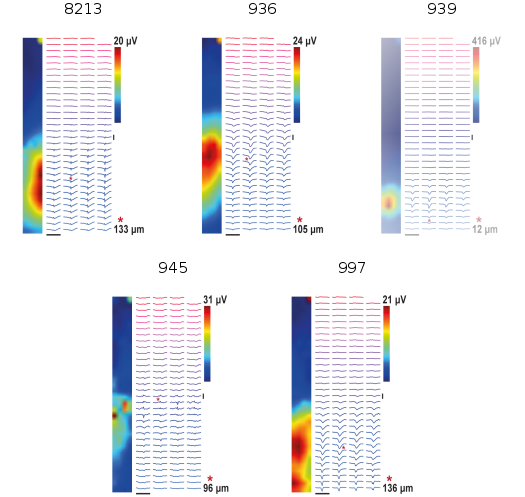
\includegraphics[width=\textwidth]{2.Chapter/dataset-JTA.png}
	\caption{Presentation of the recording used in this project. Here are presented the spatial distribution of the peak-to-peak amplitude of the Juxta-Triggered Averages, illustrated as a interpolated heatmap. In addition, the extracellular JTA waveforms for all the extracellular electrodes are spatially arranged
}
\label{fig:recordings-summary}
\end{figure}


\begin{table}[!h]
\centering
\begin{tabular}{cccccc}
\textbf{Recording ID} & \textbf{Short ID} & \textbf{Distance ($\mu m$) } & \textbf{P2P ($\mu V$)} & \textbf{Depth ($\mu m$)} & \textbf{\# Juxta spikes}\\ \hline
2015\_09\_09\_Pair7.0 & 997 & 136.2 $\pm$ 40 & 20.7 & 1032.8 & 1082  \\ 
2015\_09\_04\_Pair5.0 & 945 & 96.1 $\pm$ 40 & 30.8 & 1185.5 & 185  \\
2015\_09\_03\_Pair6.0 & 936 & 153.3 $\pm$  40 & 24.1 & 1063.2 & 3329 \\
2015\_09\_03\_Pair9.0 & 939 & 11.5 $\pm$  40 & 416.3 & 1152.8 & 5007  \\
2015\_08\_21\_Pair3.0 & 8213 & 132.8 $\pm$ 40 & 19.4 & 1286.0 & 8117 \\ 
\end{tabular}
\caption{Information about the recordings used. The values on the "Recording ID" are conform the dataset provided by \cite{Netoetal}. For convenience, a Short ID will be used throughout this document. P2P stands for Peak-to-Peak Amplitude calculated as the maximum value across electrodes of the difference between the maximum and minimum values of the JTA. In the fifth column are the values of the depth in the cortex. In the last column are the number of spikes detected in the signal from the Juxtacellular pipette.}
\label{tab:sum-recordings}
\end{table}
%$\max_i \left( \max_t \left( JTA_i \right) - \min_t \left( JTA_i \right)\right), i=0,\ldots , 127$
We have some variability in this ensemble. 
The recording 939 was recorded very closed to the neuron and therefore has a very large P2P amplitude and lies above the noise; it also recorded many spikes. 
The recording 945 has a very low count of spikes and relatively low P2P amplitude. For this reason its JTA is not very well defined.
Despite its low P2P amplitude, the recording 8213 is the one with the most events, making its JTA reasonably defined.

In Fig. \ref{fig:recordings-summary}, the spatiotemporal profile of each recording is noticeable and centered around the closest electrode in the probe.


\section{Methods}
\label{sec:methods}
\subsection{Spike Detekt}
\label{subsec:spikedetekt}

To my knowledge, SpikeDetekt \cite{Rossant2016} is the spike detection algorithm that yields the best results, in reasonable human and computational time. 

To deal with the problem of overlapping spikes SpikeDetekt uses (user-provided) information about geometry of the probe. This information consists of the electrodes positions and the adjacency graph that defines "neighbour" electrodes. 

This method uses a Butterworth filter on the first stage. Then it uses a double-threshold detection: the user defines a "weak threshold" and "strong threshold". The parts of the signal whose amplitude exceeds the weak threshold must be define a contiguous region in time as well as in space (according to the adjacency graph) and at least one data point must exceed the strong threshold. This region is called a connected component. To define this region SpikeDetekt uses the flood fill algorithm (commonly used in computer vision). This approach avoids both spurious detection of noise events and prevents the same spikes from being detected more than once.
 
After detection, spike times are calculated as the center of mass of the signal that lies above the weak threshold for each channel. This results in several spike times therefore it is necessary to align the waveforms, i.e., shift each window 

With the aligned waveforms, SpikeDetekt performs Principal Component Analysis as Feature Extraction method and the three most significant components are kept. Along with this feature vector a mask vector is calculated, so that to each detected event and each channel a number between zero and one is assigned: zero if the peak amplitude of the waveform sensed by that channel doesn't reach the weak threshold and one if the peak amplitude exceeds the strong threshold. Otherwise this number is assigned according to a function of the peak amplitude, for example, a linear function.

The mask vector ensures that temporally overlapping spikes with similar feature vector are distinguishable, and treated individually.

The output of SpikeDetekt is passed through to KlustaKwik where spikes are sorted with an unsupervised learning algorithm called Expectation-Maximization algorithm. This stage defines a number of putative neurons (classes) with spikes assigned to them.

Finally, a human operator inspects the results and manually sorts if necessary.

SpikeDetekt requires the user to define many parameters prior to running: most significantly the  weak and strong thresholds.  Rossant et al. report that the optimal values for these parameters are $\theta_w = 2 \sigma_{noise}$ and $\theta_s = 4.5 \sigma_{noise}$ where $\sigma_{noise}$ is the standard deviation of the noise for each channel which is estimated as the standard deviation estimator $s_{n-1}$ of a some time windows of the filtered signal randomly chosen from the whole recording.

These values were obtained evaluating the detection performance against hybrid labeled data (data composed by several labeled dataset acquired by the same 32-channel probe). 

\subsection{phy}
\label{subsec:phy}
As of the summer of 2015, Klusta-Team made phy available. phy is a python package for python 3.4 that allows researchers to use the API from SpikeDetekt in a modular way importing only what is necessary. phy can also be run as a command-line operation.

In the context of this project, before running phy it was necessary to convert the binary data from Neto et al. into a binary file with the struture and data type that phy expects to read. The binary file must be a flat array of 16-bit integer with the following structure:

$t_1C_1 , t_1C_2, \ldots , t_1C_N, \ldots t_TC_1 \ldots t_TC_N$ %t_2C_1, \ldots t_2C_{N_channels},

The command "phy detect filename.prm" was used. The .prm file stores all the user-defined parameters necessary for phy to work. The relevant output of this command are a .kwik file (an HDF5 file with the spike times) and a .kwx file (an HDF5 file containing the extracted PCA features and the masks for each detected spike).

\subsection{Cross-Correlograms}
\label{subsec:CC}

To analyze neural activity in the brain, scientists often look into the temporal correlation of the recorded signals. If the correlation of the signal f and signal g is defined as:
\begin{equation}
\left( f * g \right) \left( \tau \right) = \int_{- \infty }^{ + \infty } f \left( t \right) g \left( \tau + t \right) dt
\label{eq:CCdefinition}
\end{equation}
where $\tau$ is called the time delay.

If the signals are uncorrelated, their correlation will appear flat. If there exists some correlation (or even causality) between the two signals their correlation will behave interestingly (not trivial), e.g., if the second neuron always spikes 1 ms after the first one, there will be a peak when $\tau = -1$.

When performing this kind of analysis, spike signals are usually represented as a sequence of times when the neuron spiked or as a time series of 0's and 1's, if a sparse representation is preferred. These are called spike trains.

This analysis is usually done by means of calculating cross-correlograms (CCs). These are the graphical form of the cross-correlation between to signals, typically in the form of histograms.

Another useful calculation is the auto-correlogram (AC) which the cross-correlograms of a signal with itself. This should have a very high count when  which is uninformative and usually omitted. It is used to verify if there are a significant number of events with delays smaller than the refractory period; if so, the detection of spikes or the sorting was faulty.

In this document, spike trains were sequences of times at which events occurred. To calculate the cross-correlograms, the two spike trains were compared by subtracting every element of one spike train to every element of the second. Then, values of this difference that were larger than a certain value (referred to as lag) were discarded. Finally the histogram of this sequence is plotted.



\section{Results}
\label{sec:chap2-results}
To be sure about the quality of the juxtacellular recording, auto-correlograms were computed for each recording (Fig. \ref{fig:AC}).
\begin{figure}[!h]
	\centering
	\includegraphics[width=\linewidth]{2.Chapter/AC.pdf}
	\caption{Auto-Correlograms for all the recordings. The size of the bins in the histograms is 1 ms and the value for the lag is 50ms.
}
\label{fig:AC}
\end{figure}

All the auto-correlograms display a usual distribution, clearly showing a gap in the interval from -5ms to 5ms, assuring that the cell never spiked twice  within a 5ms interval, which conforms with the typical values of refractory period of $2-3ms$.

It is worth noting that on the auto-correlogram corresponding to the recording 939 a second peak is resolved around $\tau = -9 ms$ and $\tau = 9 ms$.

For each recording, phy was run with the following parameters:
The data was filtered with a forwards-backwards Butterworth filter of order 3 with cutoff frequency set to 500Hz. The noise standard deviation, $\sigma_{noise}$, was evaluated in 50 excerpts of 1 second each. The weak threshold was $\theta_w = 2 \sigma_{noise}$ and the strong threshold was $\theta_s = 4.5 \sigma_{noise}$.

The results are presented in table \ref{tab:results-from-phy}.

\begin{table}[!h]

\begin{center}
\begin{tabular}{ccccc}
Recording ID & \# detected Spikes & $\sigma_{noise}$ ($\mu V$) & $\theta_W$ ($\mu V$) & $\theta_S$ ($\mu V$) \\ \hline
8213 & 148762 &  12.95 & 25.91 & 58.30 \\ 
936 & 323629 & 10.76 & 21.52 & 48.43 \\ 
939 & 265476 & 10.51 & 21.02 & 47.29 \\ 
945 & 126234 & 10.92 & 21.84 & 49.14 \\ 
997 & 156932 & 11.47 & 22.93 & 51.60 \\ 
\end{tabular}
\end{center}
\caption{Summary of the output from phy. In this table are the values of the estimated standard deviations of the noise, and the calculated weak and strong thresholds for each recording. These values were converted into $\mu V$.}
\label{tab:results-from-phy}
\end{table}

In Fig. \ref{fig:CC} are the whole-probe cross-correlograms for the recordings, where for each detected spike, all electrodes whose corresponding mask value was non-zero were used.

\begin{figure}[!h]
	\centering
	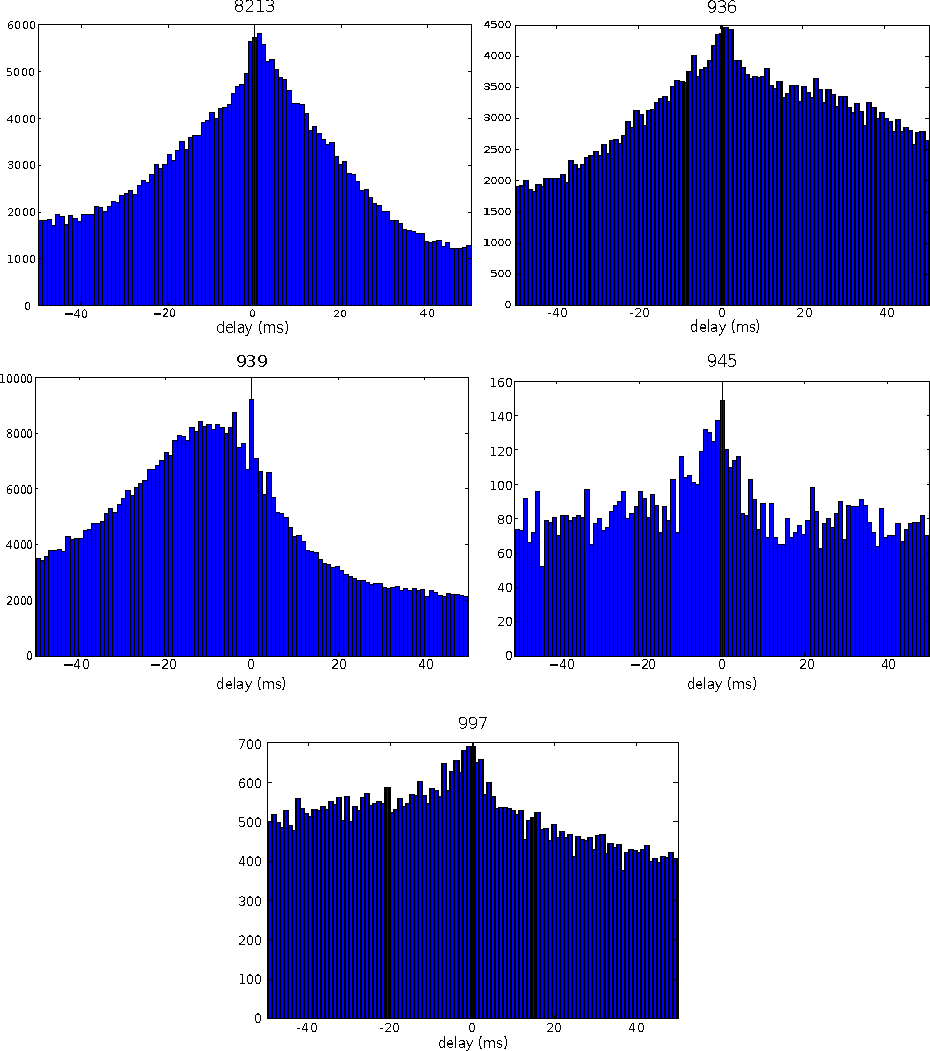
\includegraphics[width=\linewidth]{2.Chapter/CC.pdf}
	\caption{Cross-Correlograms for all the recordings. The size of the bins in the histograms is 1 ms and the value for the lag is 50ms.
}
\label{fig:CC}
\end{figure}

In Appendix A are the cross-correlograms per channel for the neuron 939, where the spike train output by phy was split according to the electrode the spike was detected on using the masks. It is noticeable that the peak only appears in some channels, which are the ones where the JTA has a larger amplitude in Fig. \ref{fig:recordings-summary}.

In Fig \ref{fig:CC}, all cross-correlograms present a somewhat coherent distribution. This means that for every value $\tau$ in the considered interval, there exists some temporal correlation between the juxta neuron and the activity of the rest of the neurons in the recorded volume. This is to be expected. According to Ruiz-Mejias et al., the use of ketamine as anesthesia in rats provokes the synchronization in the population activity in many cortical areas, including the motor cortex. This gives rise to "up" and "down" states, where most neurons in the population are firing or silent, respectively. In addition, they report that the frequency of oscillation of these states is, on average, 0.97Hz, which is close to the firing rates reported in Neto et al. 

Only on the cross-correlogram corresponding to the recording 939 can we see a distinct peak when $\tau=0 ms$, on top of the correlation with the background activity. This means that phy managed to find juxta neuron.

On the rest of the cross-correlograms in Fig \ref{fig:CC}, the peak around the central bin is never very clear. In fact, in the case of the recordings 8213 and 936, the peak is even shifted to $\tau=1 ms$. This could justify a more careful examination setting the size of the bin used in the histograms to a smaller value.

To calculate the number of events corresponding to the juxta, it is necessary to remove the counts from the correlation with the background activity. To estimate this value, the average of the counts in the bin neighboring bins ($\tau = -1ms$ and $\tau = 1 ms$) was computed and subtracted to the counts in the central bin. The results are in table \ref{tab:CCcorrection}.

\begin{table}[!h]
\begin{center}
\begin{tabular}{p{1.5cm}cccccr} %p{1.3cm}

\multicolumn{ 1}{p{1.5cm}}{Recording } & \multicolumn{ 3}{c}{Bin Counts} &  \multicolumn{ 1}{p{1.3cm}}{Corrected} & \multicolumn{ 1}{c}{Number} & \multicolumn{ 1}{c}{Accuracy} \\ 
\multicolumn{ 1}{l}{ID} & $\tau=0$ & $\tau=-1$ & $\tau=1$ & \multicolumn{ 1}{c}{Counts} & \multicolumn{ 1}{p{1.3cm}}{of JS} & \multicolumn{ 1}{l}{} \\ \hline
8213 & 5725 & 5642 & 5810 & -1 & 7760 & -0.01\% \\
936 & 4377 & 4357 & 4465 & -34 & 3329 & -1.02\% \\
939 & 9202 & 6701 & 7092 & 2305.5 & 4947 & 46.60\% \\
945 & 144 & 137 & 120 & 15.5 & 185 & 8.38\% \\ 
997 & 691 & 689 & 650 & 21.5 & 1082 & 1.99\% \\ 
\end{tabular}
\end{center}
\caption{Correction of the cross-correlograms central peak.}
\label{tab:CCcorrection}
\end{table}


In most cases, phy yields a detection accuracy close to zero. This is not surprising considering the algorithm used by phy. The maximum P2P amplitude of JTAs of these cases lies between 19.4$\mu V$ and 30.8$\mu V$ and the strong threshold is always larger than 48.43 $\mu V$. Since it is required that at least one sample in a connected component be larger than the strong threshold these spikes are never detected. Three possible explanations exist for this number of detected events. First, the neuron may have spiked simultaneously to a large noise fluctuation causing it to be detected. Secondly, the connected components of these spikes could have been connected with the connected component of other spike which exceeded the strong threshold. This would result in the detection one single spike where the computed spike time was closer to the corresponding juxta spike time and therefore contributed to the central bin in the cross-correlograms.

Even in the recording 939 the detection rate is fairly low, considering it has a very large P2P amplitude. In fact, the connect component corresponding to spikes from the juxta neuron were expected to be large and therefore may have been merged together with other spikes present in probe. In this case, all these events will only be detected as one, which leads to the relatively low count in the central bin of the cross-correlogram of this recording.

To illustrate this, the masks of the events that occurred closest to the juxta spikes were calculated. Examples of these mask are in Fig. \ref{fig:masks-examples}.
 
\begin{figure}[!h]
	\centering
	\includegraphics[width=\linewidth]{2.Chapter/masks-939-ready.pdf}
	\caption{Examples of masks on the events whose assigned times (on top of each plot, in ms) is closest to the times from the juxta neuron.
}
\label{fig:masks-examples}
\end{figure}

The average of these masks is presented in Fig. \ref{fig:masks-average-std}. The maximum value for the standard deviation of the average was $6.0 \times 10^{-3}$ which is very low and therefore it is fair to say that most of the masks of the juxta spike are in this collection.

\begin{figure}[!h]
	\centering
	\includegraphics[width=0.5\linewidth]{2.Chapter/average-and-std-mask-939.pdf}
	\caption{Average mask and its standard deviation of the events whose times were closest to the times from the juxta neuron.
}
\label{fig:masks-average-std}
\end{figure}


Looking at the mask of the events on times 86.5 ms  and 100.1 ms it is clear that there are connected components from two spikes other than the one from the juxta neuron that were merged together. This situation could possibly be solved by increasing the weak threshold, however this would lead to an increase of false negatives. 
%%%%%% Another possibility would be performing multimodal analysis to separate the different connect components.

In this chapter, using the ground-truth data from Neto et al. it was possible to identify some of the issues and limitations of the SpikeDetekt algorithm. On the next chapter a different approach is presented and evaluated.

%\section{Section B}
\label{sec:sectionb}

\subsection{Subsection A}
\label{subsec:subasectionB}

The model described can also be represented as

\begin{equation}
\dot{\mathbf{x}}(t) = \mathbf{T}\mathbf{z}(y),\  \mathbf{y}(0) = \mathbf{y}_0,\  z\geq 0 \\
\label{eq:dummyeq1}
\end{equation}

\noindent where

\begin{equation}
\mathbf{A} = \left[ \begin{array}{cc} -(a_{12} + a_{10}) & a_{21} \\ a_{12} & -(a_{21} + a_{20}) \end{array} \right],\ \mathbf{x} = \left[ \begin{array}{c} x_1 \\ x_2 \end{array} \right] \\
\label{eq:dummyeq2}
\end{equation}


\subsection{Subsection B}
\label{subsec:subbsectionB}

\begin{table}[H]
	\centering
	\caption{Dummy Table.}
	\begin{tabular}{|c|c|c|c|} \hline
		\textbf{Vendor Name} 				& \textbf{Short Name}	& \textbf{Commercial Name}	& \textbf{Manufacturer}	\\ \hline \hline
		\multirow{3}{*}{Text in Multiple Row}		&	ABC				&  ABC\textreg				& ABC SA			         \\ \cline{2-4}
		 								&        DEF				&  DEF\textreg				& DEF SA				\\ \cline{2-4}
										&        GHF			&  GHF\textreg				& GHF SA				\\ \hline
		Text in Single Row					&        IJK				& IJK\textreg				& IJK SA				\\ \hline
		Frescos SA						&        LMN			& LMN\textreg				& LMN SA				\\ \hline
		Carros Lda.						&    \multicolumn{3}{|c|}{Text in Multiple Column}							\\ \hline
	\end{tabular}
	\label{tab:dummytable}
\end{table}
\cleardoublepage

% %%%%%%%%%%%%%%%%%%%%%%%%%%%%%%%%%%%%%%%%%%%%%%%%%%%%%%%%%%%%%%%%%%%%%%
% Dummy Chapter:
% %%%%%%%%%%%%%%%%%%%%%%%%%%%%%%%%%%%%%%%%%%%%%%%%%%%%%%%%%%%%%%%%%%%%%%

% %%%%%%%%%%%%%%%%%%%%%%%%%%%%%%%%%%%%%%%%%%%%%%%%%%%%%%%%%%%%%%%%%%%%%%
% The Introduction:
% %%%%%%%%%%%%%%%%%%%%%%%%%%%%%%%%%%%%%%%%%%%%%%%%%%%%%%%%%%%%%%%%%%%%%%
\fancychapter{Deep learning}
\label{cap:chapter3}

\textit{Present the chapter content.}

%\input{2.Chapter/Chap2-Introduction.tex}
To address the issues presented in the previous chapter and to take advantage of the labeled paired recordings in Neto et al.,

In order to overcome the issues presented in the previous chapter, a different approach was tried. In this chapter is report the attempt of employing recent techniques of deep learning to perform spike detection.


\section{Introduction}
For millennia, humans (and other animals) have tried to understand the rules that govern the phenomena surrounding them based on observations. This knowledge allowed them to expand the reach of their predictions and develop inventions to improve their way of living, as well as the empirical laws that support all the fields of fundamental science, and consequently applied science. In the last 5 decades, with the advent of several kinds of sensors, fast electronics and large storage capacity, quantitative observations have become more and more numerous at a great level of detail (the "deluge of data") and it appears that this way of learning is becoming more and more necessary in the present than ever before.

Datasets became very large in the number of elements as well as very high in their dimensionality (the "Deluge of Data"), in such a way that they are no longer amenable for a human operator to analyze them directly. To be able to deal with this problem, researchers and engineers started using computers in particular methods of Machine Learning. Machine Learning is a subfield of computer science that studies and develops algorithms meant to find new structures or rules a given experiment or phenomenon is based on. Arthur Samuel defined machine learning as a "Field of study that gives computers the ability to learn without being explicitly programmed".

However, conventional machine learning techniques often require careful and domain-specific design in order to achieve good results. For example, it usually takes a considerable amount of expertise and experience with a phenomenon of interest in order to determine an algorithm and/or model that would be a good approximation of what was actually happening in the experiment under study.

In the field of statistical machine learning, a dataset consists of m points (examples), each one with a set of n features defining a n-dimensional space (input space). Depending on the specific kind of model we would like to extract from the data, there are a number of different approaches for machine learning.

\section{Methods}

The most commonly used form of machine learning uses labeled datasets. This is called supervised learning.

\subsection{Supervised Learning}
\label{subsec:supervised-learning}

In supervised learning, each input example has an extra feature that represents the “true” value, the "right answer" we would like to obtain from the machine for this instance. If the dataset has such features, it is said to be labeled, otherwise, it is unlabeled.

Supervised learning algorithms are usually iterative methods. They are usually presented with a large number of labeled examples beforehand, which they then use to modify the evaluation model in order to output the best possible answer. These modifications follow a set of operations (the training or learning algorithm), that depends on some measure of dissimilarity between the outputs of the model in its current configuration (the model predictions) and the corresponding labels. This function is usually called a loss function and is most often thought of as a distance. Examples of loss functions are the Mean-Squared Error of Cross Entropy. At each iteration, the training algorithm will calculate the necessary adjustments in order to make the loss function smaller. After a certain number of iterations, the algorithm will, possibly, converge on a solution that is a good enough approximation of the results a human supervisor would produce when analyzing the same dataset.

In machine learning, we must choose a model (or framework) to work with. In the case of linear regression, the output of the algorithm is a linear function of the form $y = mX + b$, where m and b are the adjustable parameters. This choice strongly conditions the power of the algorithm. If, for instance, y depends on $X$ quadratically, linear regression may not yield the best results; however, depending on the situation it may provide a good enough approximation.
Another choice the user must define a priori is the training algorithm. A simple example of such an algorithms is gradient descent. 

In supervised learning we are not only interested in producing a model for the data we do have but more generally in predicting the outcome of the experiment in untested situations that we have yet to observe.

More formally, the computer receives a number, m, of examples of input as a (n-dimensional) feature vectors $\vec{x_i}, i = 1,2, \ldots ,m$ and corresponding (p-dimensional) target (“true”) value $\vec{ y_i}, i=1,2, \ldots ,m$ and tries to find the element in the family of functions (hypothesis class) $h_{\theta}$ parameterized by $\theta$ such that $\vec{ y_i}  \approx h_\theta \left(\vec {x_i} \right)$ for each example. 

\subsubsection{Linear Regression}
\label{subsubsec:linear-regression}
In the context of linear regression, we restrict ourselves to a family of function such that:
\begin{equation}
h_{\vec{\theta},b} ( \vec{x} ) = \sum_{j = 1}^{m} \theta_j x_j + b = \theta \cdot \vec{x} + b
\end{equation}
where $\theta$ and $b$ are the parameters to be learnt.

A common choice for the loss function is the Mean Squared Error (MSE), defined as:

\begin{equation}
J \left( \theta , b\right) = \frac{1}{2} \sum_{j=1}^m \left[ h_{\theta,b} \left( \vec{x}^{(j)} \right) -  y^{(j)} \right]^2 =  \frac{1}{2} \sum_{j=1}^m \left( \theta \cdot \vec{x}^{(j)} + b - y ^{(j)} \right) ^2
\label{eq:MSE-definition}
\end{equation}

Most training algorithms require the knowledge of the gradient of the loss function with respect to the model's parameters to determine the update rule. In this situation, the gradient would be:

\begin{eqnarray}
\frac{ \partial J}{\partial \theta_i } &=& \sum _{j= 1}^m x_i^{(j)} (  h_{\theta, b} ( x^{(j)}) - y^{(j)} ) \\
\frac{ \partial J}{\partial b } &=&  \sum _{j= 1}^m (  h_{\vec{\theta}, b} ( x^{(j)}) - y^{(j)} )
\label{eq:MSE-gradient}
\end{eqnarray}

And the parameters would be updated as:
\begin{eqnarray}
\theta_i^{n+1} &=& \theta_i^{n} - \eta \left[\nabla_{\theta} J(\theta^n,b^n )\right]_i \\
b^{n+1} &=& b^n - \eta \frac{\partial J}{\partial b} \left(\theta^n,b^n \right)
\label{eq:GD-update-rule}
\end{eqnarray}
where $\eta$ is the learning rate defined by the user.


\subsubsection{Logistic Regression}
\label{subsubsec:Logistic-Regression}
Machine learning is also often used to perform a classification task where we are trying to assign a class (discrete value) to some input vector. For instance, we could apply linear regression and set a  threshold value to define the boundary between two class. However this method is very sensitive to extreme values of the input. In the case of binary classification $y^{(i)}$ can only be either 1 or 0. In this situation Logistic Regression is usually a better choice. With logistic regression we try to find the predictor choosing a different hypothesis class: 
\begin{equation}
h_{ \theta, b } (x) = \sigma ( \theta \cdot x + b) = \frac{1}{ 1 + exp(-\theta \cdot x - b) }
\label{def:logistic-regression}
\end{equation}
Note that this function (called the sigmoid function or logistic function) is a continuous for all values of $x$. It is always positive, monotonically increasing from zero to one. This leads to the interpretation of the output of the logistic regression as the probability of the class labeled as “1” happening given the input vector x: 
\begin{eqnarray}
P( Y=1 \mid  X = x ) &=& \frac{1}{ 1 + \exp(-\theta \cdot x - b)} \leqslant 1 \\
P( Y=0 \mid  X = x ) &=& 1 - P( Y=1 \mid  X = x )
\end{eqnarray}

The cost function in this case is usually defined as:
\begin{equation}
J(\theta,b) = - \sum _{j= 1}^m ( y^{(j)} \log(h_{\theta,b}(x^{(j)})) + (1-y^{(j)}) \log(1- h_{\theta,b}(x^{(j)})) )
\end{equation}

Since in this setup $y^{(j)}$ can only be either 1 or 0, only one of the terms inside the summation is non-zero.

The gradient of this loss function is:
\begin{equation}
\nabla _{\theta,b} J(\theta,b) = \sum _{j= 1}^m x^{(j)} ( h_{\theta,b}(x^{(j)}) - y^{(j)} )
\end{equation}

In classification tasks it is common to have more than two classes that we are interested in. In this case, we can generalize logistic regression to many-classes using Softmax Regression, where the probabilistic interpretation is applied

In classification task, we are looking for the boundary between classes in the feature space. The techniques I mentioned above can only resolve problems in which the classes are linearly separable (where the boundary is an hyper-plane in the feature space). But this is not always the case. Sometimes the region corresponding to a particular class may even be disjoint. In such case linear classifiers are not powerful enough to solve the problem. (As an example consider the Exclusive OR function where the inputs are two binary valued variables. There is not straight line in the input space that separates the class “0” and the class “1”.)

\subsection{Artificial Neural Networks}
\label{subsec:ANN}

A much more powerful concept is that of Artificial Neural Networks. 
An artificial neuron (hereafter neuron unless stated otherwise) is a computational unit that takes as input the vector $x$ and outputs
\begin{equation}
h_{w,b} (x) = f\left( w \cdot x + b \right) = f \left( \sum_{i=1}^n w_i x_i + b  \right)
\end{equation}

where $f\colon \textbf{R} \rightarrow \textbf{R}$ is called the activation function. The vector $\textbf{w}$ and the value of b (called the bias or intercept term), as before, can be tuned according to some algorithm to perform a designated task as good as possible. 

If the activation function is the sigmoid function we recover the logistic regression.

Another example of activation function is the hyperbolic tangent, which increases from -1 to 1. 
Lately, researchers and engineers have started using the rectified linear function (RELU) particularly in the context of deep neural network (which I'll talker later in this document). This function is defined as
\begin{equation}
RELU(z)= \max(z,0) = 
\begin{cases}
    z,& \text{if } z\geq 0\\
    0,              & \text{if } z < 0
\end{cases}
\end{equation}

This activation function is significantly different from the ones referred before because it is not bounded as $z$ increases. Moreover, it is not differentiable when $z=0$ although this doesn't become a problem in practice because it is differentiable at any point arbitrarily close to 0.

A Artificial Neural Network (ANN) is put together by hooking together many of these simple neurons by means of function composition where the output of one neuron is the input of another.


\begin{figure}[!h]
	\centering
	\includegraphics[width=0.7\linewidth]{3.Chapter/firstANN.pdf}
	\caption{Graphical visualization of an illustrative example of an artificial neural network. This ANN is composed by three layers with three neurons on the first two and one neuron on the output layer. The connections between all the neurons are also represented, in addition to the connection to the bias term represented by the extra nodes on the bottom with the label "+1".
}
\label{fig:first-ANN}
\end{figure}
In the Fig. \ref{fig:first-ANN} is a graphical representation of what was just mentioned. On the left, we have the input layer (layer $L_1$) where the input vector $(x_1,x_2,x_3)$ is fed. In the middle there are three neurons. These are called hidden neurons and they compose one hidden layer ($L_2$). Finally, there is the output layer with only one neuron. There are also two nodes on the bottom that represent the bias term.

In this example, there are connections between all neurons of one layer to the neurons in the next layer. This ANN is said to be fully connected (or densely connected). For each connection there is an associated parameter (weight) and also a bias parameter. The input of each neurons in the hidden layer is a linear combination of the output of the neurons in the previous layer weighted by the parameters of the corresponding connections and summed with the bias term. In this case, the weights for the connections coming in to the first neuron in the layer L2 are $w_{1,1}^{(1)},w_{1,2}^{(1)},w_{1,3}^{(1)}, b_1^{( 1 )}$ and its input is:
\begin{equation}
z_1^{(2)} = \sum_{i=1}^3 w_{1,i}^{(1)} a_i^{(1)} + b_1^{(1)}
\end{equation}
This input is then fed into the activation function which reveals the outputs of this neuron as 
\begin{equation}
a_1^{( 2 )} = f\left( z_1^{(2)} \right)
\end{equation}

We denoted the number of layer as $n_l$ and the number of neurons in the layer $L_l$ as $S_l$. In the example above $n_l=3$, $S_1 = S_2 = 3$ and $S_3 = 1$

In general, when the network is densely connected, the input of the neuron i in the layer j is:
\begin{equation}
z_i^{(j)} = \sum_{k=1}^{S_{l-1}} w_{i,k}^{(j)} a_k^{(j-1)} + b_i^{(j-1)}  
\end{equation}
And its output is:
\begin{equation}
a_i^{(j)} = f(z_i^{(j)})
\end{equation}
It is also convenient to introduce a matrix notation such that:
\begin{equation}
\textbf{z}^{(j)} = \textbf{W}^{(j)} \textbf{a}^{(j-1)} + \textbf{b}^{(j-1)}
\end{equation}
where the vector $\textbf{z}^{(j)}$, $\textbf{a}^{(j)}$ and $\textbf{b}^{(j)}$ represent the input, output and bias parameter of all neurons in Layer $L_j$

The output of the output layer is denoted $\textbf{h}_{\textbf{W},\textbf{b}}\left( \cdot \right) = \textbf{a}^{(L)}\left( \cdot \right)$


Using Artificial Neural Networks, we now have a much more powerful and flexible framework to create models that can be trained to compute much more complex functions than the ones computable with traditional machine learning algorithms.

However, there's still the need to define the training algorithm. In order to use the gradient descent algorithm, it is necessary to compute the gradients of the loss function with respect to all the adjustable parameter of ANN. These gradients are usually computed using the back-propagation algorithm. In this method, the label is subtracted from the output value as an estimate of the gradient on the output layer. This value is then propagated backwards layer by layer by applying the chain rule for derivatives, which will depend on the chosen activation functions. With the gradients estimated, the parameters are update in the way defined earlier in equation \ref{eq:GD-update-rule}

The key aspect of learning with ANN is that, due to its generalization power, the form of the final output function is not directly designed by a human: they are learned from the data.

But this framework leads to questions of how exactly to define the model. In other words, how to define the architecture of the ANN, i.e., how many neurons should there be in the ANN and how should they be connected? There are two basic topologies: shallow networks and deep networks. In shallow networks, there is at most one hidden layer, whereas a network is said to be deep if it has two or more hidden layers. This distinction has become very important over the last three decades. On the one hand, it has been shown that a shallow ANN with only one arbitrarily large hidden layer could approximate a function to any level of precision (\cite{hornik1989multilayer}). Nonetheless, this level of precision would only increase with exponentially increasing number of neurons, becoming computationally very demanding.

On the other hand, deep neural networks are conceptually more interesting because each layer can be thought of as a representation of the input in a higher and higher level of abstraction, similar to how the visual processing hierarchy in cortex is thought to operate to construct human visual perception. However, using back-propagation and gradient descent with the usual sigmoid or tanh function can very quickly run into the problem of “vanishing gradients”, when the activation function saturates and the training will not proceed any further. Moreover, even in the cases where training is possible, deep networks were originally found to perform worse than shallow networks. \cite{NNDL} \cite{Larochelleyoutube}

However, in the past decade there have been several theoretical and technological advances that brought deep neural network back to life.

\subsection{Deep Learning}
\label{subsec:Deep-Learning}
Representation learning is a family of methods that allows machines to find new ways of representing the raw data it was fed with. Deep Learning tries to accomplish this in a "layer by layer" manner. In a deep neural network, each layer holds a new representation of the input data, by transforming the output of the previous layer into a new representation, a more abstract way of perceiving the input data. Composing many of these layer, it should be possible to compute very complex function. For the case of classification task, higher layers of representation may amplify aspects of the input that are important for the discrimination and suppress irrelevant features.

In this section, the techniques used in this project will presented such as training (or optimization), loss function, initialization methods and regularization

\subsubsection{Stochastic Gradient Descent}
\label{subsubsec:SGD}
Stochastic Gradient Descent (SGD) is a stochastic approximation of the gradient descent algorithm described in the previous section. In SGD, only utilizes a subset (called a batch) of the provided examples to compute the gradient. This "noisy" approximation of the gradient is then used to update the parameters of model. It should be noted that all the examples in the dataset are utilized: the entire dataset is split in batches and for each batch there is one update in the parameters. One pass through the entire dataset is called an epoch. This means that there will be more (but faster) iteration than in the standard gradient descent. Surprisingly, this simpler method is known to yield good results much faster than more sophisticated algorithms.

Stochastic learning is often much faster than classic learning particularly when using large redundant datasets: if, for instance, the dataset is composed of the ten repetitions of a smaller set of examples, then estimating the gradient using the whole dataset would have the same result as using one tenth of the dataset. Of course in practice two examples are rarely the same. However many example may be acquisition of the same pattern and therefore will contain approximately the same amount of information.

Networks learn the fastest from examples that are most distant from what the network predicted. Therefore it would preferable to choose such examples in each iteration. Of course, there is no simple way to know which are the "good" examples to train the network with in each iteration. There is a relatively simple way of applying this idea. Assuming successive examples do not differ much, shuffling the dataset before splitting would make the batches "richer" in terms of the information they contain.

Another interesting characteristic of stochastic learning is that it is less prone to get the network stuck in local minima of the loss function. The noise introduced in the gradient estimation generates updates on the parameters that allow easier "jumps" of the parameters from one local minima to another, possibly deeper than the previous. On the other hand, this noise also prevents the full convergence to the minimum: the parameter will always have stochastic fluctuation. This can be address by  adaptively changing the size of the batch or the learning rate.

\subsubsection{AdaGrad}
\label{subsubsec:Adagrad}
One solution for the problem just mentioned is AdaGrad (Adaptive Gradient optimization), proposed in 2011 by Duchi et al. \cite{duchi2011adaptive}. In this algorithm, the learning rate is adapted in each iteration according to the geometry of the loss function in the vicinity of the current values of the parameters. For each element in the parameter matrix, the user-defined learning rate $\eta$ is weighted by factor that makes it larger or smaller according to a (fast) approximation of the Hessian Matrix. In other words, the update for each parameter is more coarse when far from a local minimum and finer when close to a local minimum.

It should be noted that this algorithm was proposed for convex optimization problems. However, even in non-convex situations AdaGrad usually performs better that standard SGD.\cite{gupta2014training}

\subsubsection{Parameter Initialization}

The starting values of the weights can have a significant effect on the training process. For instance, in an ANN with the hyperbolic tangent as activation function, if all parameters were initialized with the same value all neurons would output the same value and get the same updates during training. This would render the network useless. For this reason it is necessary to break these symmetries from the onset.

To get the most out a certain ANN, the initial parameters should be as  uncorrelated as possible. However, if the weights are initialized with very high values, a sigmoid or tanh activation function would start saturated, gradients would vanish and the training wouldn't be possible.
To solve this problem, the initial parameters are usually  sampled from a uniform distribution $U([-a,a])$, where a is some small value. There are several proposals for determining the value of a depending on the particular model chosen by the user: He Uniform \cite{he2015delving}, Xavier Uniform \cite{glorot2010understanding} (also known as Glorot Uniform) or LeCun Uniform \cite{lecun2012efficient}.

For example, LeCun Uniform was defined with sigmoid activation functions in mind. With this initialization method, starting values for the weights are drawn from a uniform distribution with zero mean and standard deviation such that the input of each neuron has a standard deviation close to 1.

\subsubsection{Loss Function}
\label{subsubsec:loss-function}

As mentioned above, most optimization algorithms (as is the case of SGD) try to minimize a loss function. There are many ways to define this function. One possible way is using the Mean Squared Error as explained in \ref{subsubsec:linear-regression}. However in classification tasks the output of the classifier is usually interpreted as the probability of a certain input belonging the a certain class. With this in mind, it is possible to define a loss function as the distance between the desired probability distribution and that of the output of the classifier in the current configuration. This can be done by means of the cross-entropy. In the case of a binary classification, the (not normalized) cross-entropy is estimated from the samples as:
\begin{equation}
H = - \sum_j \left( y^{(j)} \log h_{W,b} \left( x^{(j)} \right) + (1 - y^{(j)}) \log \left( 1 - h_{W,b}\left( x^{(j)} \right) \right) \right)
\end{equation}
where $y^{(j)}$ can only take the values 0 or 1 and therefore only one of the terms will be non-zero. When the classifier outputs the right answer the logarithm will tend to zero and so will the penalty corresponding to that data point. \cite{murphy2012machine}

\subsubsection{Regularization}
The role of regularization is to penalize certain types of function to emerge during the training process. In particular, we are interested in penalizing functions that are too complicated and too non-linear that would overfit the training set.

This is usually done by adding an extra term, $\Omega \left( W \right) $, to the loss function that depends on the value of the weights of the connections between neurons; the bias terms are not usually regularized.

A common choice is the $L_2$ regularizer where the extra term is the $L_2$ norm of $\mathbf{W^{(k)}}$:
\begin{equation}
\Omega \left( \mathbf{W} \right) = \sum_k \sum_i \sum_j \left( W_{ij}^{(k)} \right)^2 = \sum_k |\mathbf{W^{(k)}} | ^2
\label{eq:L2-reg}
\end{equation}

The gradient of this term with respect to the weights is:
\begin{equation}
\nabla_{\mathbf{W^{(k)}}} \Omega \left( \mathbf{W} \right) = 2 \mathbf{W^{(k)}}
\label{eq:L2-reg-grad}
\end{equation}

Another option is to use the $L_1$ norm instead. The regularization term takes the form:
\begin{equation}
\Omega \left( \mathbf{W} \right) = \sum_k \sum_i \sum_j | W_{ij}^{(k)} |
\label{eq:L1-reg}
\end{equation}
which leads to the gradient:
\begin{equation}
\nabla_{\mathbf{W^{(k)}}} \Omega \left( \mathbf{W} \right) = sign \left( \mathbf{W^{(k)}} \right)
\label{eq:L1-reg-grad}
\end{equation}
when $w_{ij}^{(k)} \neq 0$

Unlike the $L_2$-regularization, this gradient does not vanish as the value of $w_{ij}^{(k)}$ approaches zero. Therefore, in this case there is a stronger tendency to got parameters that are very small, allowing for the interpretation of these connections as non-existent, decreasing the resulting complexity of the network.

The relative importance of the regularization term is controlled by an hyperparameter $\lambda$ called the weight decay. When $\lambda$ is set too high the training algorithm will "prefer" minimizing the magnitude of the parameters over making output closer to the labels. If $\lambda$ is too low, the optimizer is likely to train the network into overfitting the training set. \cite{Larochelleyoutube}

Another way of dealing the problem of overfitting is using stochastic dropout training.
The term "dropout" refers to dropping out units (mostly hidden units) in a neural network. Dropping out means temporarily removing certain neurons from the network, along with all its incoming and outgoing connections. The choice of which units to drop is random. In the simplest case, each unit is retained with a fixed probability p independent of other units, where p can be chosen the user.
In other words, in each epoch at training time, a fraction p of units from a certain layer is "forgotten". This results in a smaller temporary network. Then the usual training (forward propagation and back propagation) is performed in this subnetwork. The value of p can be different for each layer.
With this procedure, a unit cannot "assume" that all units will be present in each epoch, so it cannot co-adapt to other units. This way each neuron is forced to extract feature that are useful generally and not only when used in combination with other units.
At test time, the output of each unit is multiplied by the corresponding value of p. \cite{Hinton2012} \cite{srivastava14}

\section{Results}
\label{sec:DL-results}

\subsection{Hardware and Software setup}
\label{subsec:hardware-software}
To implement the neural networks I used Keras \cite{chollet2015keras}. Keras is Artifitial neural network library written in python programming language. It is designed to be minimalistic, modular and straight forward to use, but yet powerful and generic enough to build serious models. It is built on top of either Theano or Tensorflow. In this work, I used the Theano backend. Theano is a Python library that lets you to define, optimize, and evaluate mathematical expressions, especially ones with multi-dimensional arrays (numpy.ndarray). Using Theano it is possible to attain speeds rivaling hand-crafted C implementations for problems involving large amounts of data. It can also surpass C on a CPU by many orders of magnitude by taking advantage of recent GPUs, using the latest version of CUDA platform. \cite{theano2010} \cite{theano2012}

The work reported in the following sections were performed under the following hardware setup:
\begin{itemize}
\item Microsoft Windows 8.1 Pro (64-bit)
\item Intel Core i7-3770 CPU
\item 32.0GB of RAM
\item GeForce GTX 660 video card
\end{itemize}

\noindent 
and the following software setup:
\begin{itemize}
\item python 3.4.4
\item numpy 1.10.4
\item keras 0.3.2
\item theano 0.8.0dev0
\item CUDA 7.5
\end{itemize}

Only one GPU was utilized when performing the computations in this chapter, however it is worth noting that as of March 2016 Theano added support for multiple GPUs.

\subsection{Data Preparation}
\label{subsec:data-preparation}
The same datasets from the previous chapter were used. First it was necessary to prepare the data to be fed to the DNN.Each dataset was first filtered using the same filter as phy: a forwards-backwards Butterworth filter of order 3 with cutoff frequency set to 500Hz. Each dataset was then normalized dividing by its maximum value, such that every sample has a value between -1 and 1.

Each example was defined to be the array of time windows of 100 samples for each of the 127 channels in the probe. Therefore, the input data has 12700 dimensions. However, due to constraints on the available hardware, not all windows were used. Each window is shifted by 5 samples from the previous one, i.e., the first example are the 127 time windows with $t \in [ 0 , 99]$ and the second example are the 127 time windows when $t \in [ 5, 104]$. Furthermore, only samples in $t \in [1000000,2000000]$ were utilized. This yields, at this stage, 199980 examples per dataset

The windows whose central sample was closer to the Juxta Times were labeled as "1" (positive examples). Otherwise they were labeled as "0" (negative examples). The label "1" should be interpreted as "contains a spike from the juxta cell" and "0" as "doesn't contain a juxta spike". It is possible that a spike from the juxta cell be partially contained in the window of another spike from the juxta cell. However this situation is highly unlikely since for that to happen it would mean that the two spike were separated by less that 50 samples, corresponding to 1.67 ms which is less than the refractory period of cells under consideration.

This input data was split in two set: the training set (TS), with which the DNN will train, and the validation set (VS), where the resulting trained DNN is tested. The TS held 70\% of the input data (139986 examples) and VS held the remaining 30\% (59994 examples)

In table \ref{table:summary-beforeUS} is result of this splitting.
\begin{table}[htbp]
\begin{center}
\begin{tabular}{r|cc|cc|cc}
\multicolumn{1}{l|}{} & \multicolumn{ 2}{c|}{Input Data} & \multicolumn{ 2}{c|}{Training Set} & \multicolumn{ 2}{c}{Validation Set} \\ \hline
cell ID & No. of "1"  & Fraction & No. of "1"  & Fraction & No. of "1" & Fraction \\ \hline
8213 & 292 & 0.15\% & 202 & 0.14\% & 90 & 0.15\% \\ 
936 & 127 & 0.06\% & 83 & 0.06\% & 44 & 0.07\% \\ 
939 & 298 & 0.15\% & 207 & 0.15\% & 91 & 0.15\% \\ 
945 & 14 & 0.01\% & 9 & 0.01\% & 5 & 0.01\% \\ 
997 & 38 & 0.02\% & 29 & 0.02\% & 9 & 0.02\% \\ 
\end{tabular}
\end{center}
\caption{In this table are presented, for each recording, the number of examples labeled as "1" and its fraction in the Input Data, and separated in the Training Set and Validation Set. The total number of examples in the Input Data, Training Set and Validation Set are 199980, 139986 and 59994, respectively}
\label{table:summary-beforeUS}
\end{table}

As can be seen in in Table \ref{table:summary-beforeUS}, all recordings reveal a very large unbalance: there are always many more examples belonging to the class "0". In these situations, the most likely scenario is the convergence of the DNN to a trivial solution where it outputs "0" regardless of the input, yielding an accuracy equal to the fraction of examples labeled as "0".

To address this problem, it was necessary to perform upsampling: the positive examples were repeated by the same factor in both the TS and the VS. The upsampling factor was determined so that the positive examples represent around 30\% of the total number of examples in both the TS and the VS.

The results of the operation are presented in table 

\begin{table}[htbp]
\begin{center}
\begin{tabular}{c|ccc|ccc}
\multicolumn{1}{l|}{} & \multicolumn{ 3}{c|}{Training Set} & \multicolumn{ 3}{c}{Validation Set} \\ \hline
cell ID & No. of ex. & No. of "1" & Fraction & No. of ex. & No. of "1" & Fraction  \\ \hline
8213 & 195334 & 55550 & 28.4\% & 84654 & 24750 & 29.2\% \\ 
936 & 192276 & 52373 & 27.2\% & 87714 & 27764 & 31.7\% \\ 
939 & 195669 & 55890 & 28.6\% & 84473 & 24570 & 29.1\% \\ 
945 & 191412 & 51435 & 26.9\% & 88564 & 28575 & 32.3\% \\ 
997 & 201060 & 61103 & 30.4\% & 78948 & 18963 & 24.0\% \\ 
\end{tabular}
\end{center}
\caption{In this table are presented the total number of examples and the number of examples labeled as "1" as well its fraction on the Training Set and Validation Set after upsampling was performed. }
\label{table:summary-afterUS}
\end{table}

This procedure artificially increases the size of datasets. However the resulting sizes are relatively close to each other and therefore DNNs trained with all the TS can be compared fairly.

\subsection{Basic Model}
In this project, we planned to study how a  feed-forward deep Neural Network performs as a spike detection for neural data. In the context of machine learning this is a binary classification problem.

It was necessary to define the basic architecture of the DNN. First and foremost, the dimension of the input layer was set to 12700 and the output layer should have only one neuron.
Usually the number of adjustable parameters in a DNN should be of the same order of magnitude of the number of examples to be used and therefore the following layer had to be much smaller. In fact, to follow this rule, the second layer should have around 15 neurons. This would be 800-fold compression which seemed excessive. Therefore, it was necessary to compromise. The second layer was define with 200 neurons. Comparatively the size of the following layer had very little influence and for that reason it was decided not to compress any further and set the dimension of layer 3 and 4 to have 200 neurons as well. 

Following the results of \cite{glorot2011deep} Rectified Linear Units (RELU) were chosen as the activation function, which should result in faster learning and weaker dependence on the initial conditions. For the last layer a sigmoid activation function was used, since the problem under consideration is a binary classification.

As for the loss function, cross entropy was chosen given its characteristic fast converge.

The training algorithm was chosen to be AdaGrad.
Regarding the regularization method, the L1-norm was utilized as well as dropout with probability parameter of 0.2.

This defines the basic model of DNN that was utilized: it was a fully-connected feed-forward DNN with:
\begin{itemize}
\item $n_l$ = 5
\item $S_1 = 12700, S_2=S_3=S_4 = 200, S_5=1$
\item ReLU as activation function for hidden units and Sigmoid for the output neuron
\item Adagard as the training algorithm
\item Cross-entropy for loss function
\item L1-Regularizer along with dropout
\end{itemize}

\subsection{Optimal Hyperparameters}
\label{subsec:hyperparameters}

When defining the model to be trained some choices must be made, and there aren't exact ways of making those choices. Some are relatively straight-forward as some of the ones in the previous section. However, there are some parameter that are not as easy to set and therefore we're forced to study their influence on the performance of the DNN.

At this point, we still have to define:
\begin{itemize}
\item The size of the batch used by AdaGrad
\item The "standard" learning rate
\item The weight decay
\item The initialization method
\end{itemize}

First, the batch size was set to 10000, to be as large as the computer memory could handle.

Using the recording 939, the basic DNN was trained with different sets of parameters. 


To study the learning rate, the weight decay was set to $\lambda = 0.001$ and the initialization method was LeCun Uniform. The learning rate was set to 0.001, 0.01 and 0.1. The results are in the Fig. \ref{fig:study-LR} and \ref{fig:study-LR-zoomed}

\begin{figure}[htb]
	\centering
	\includegraphics[width=\linewidth]{3.Chapter/study-on-learning-rates-norm.pdf}
	\caption{Study on Learning Rate. Loss function and accuracies in the training set and in the validation set.The weight decay was fixed at $\lambda = 0.001$, and the initialization method was LeCun Uniform.
}
\label{fig:study-LR}
\end{figure}

\begin{figure}[htb]
	\centering
	\includegraphics[width=\linewidth]{3.Chapter/study-on-learning-rates-zoomed-ending-norm.pdf}
	\caption{Study on Learning Rate - zoomed. Loss function and accuracies in the training set and in the validation set.The weight decay was fixed at $\lambda = 0.001$, and the initialization method was LeCun Uniform.
}
\label{fig:study-LR-zoomed}
\end{figure}

To study the weight decay, the learning rate was fixed at $\eta = 0.01$ and LeCun Uniform was used. The results are in Fig. \ref{fig:study-weightdecays} and Fig. \ref{fig:study-weightdecays-zoomed}

\begin{figure}[htb]
	\centering
	\includegraphics[width=\linewidth]{3.Chapter/study-on-weight-decay-norm.pdf}
	\caption{Study on weight decay. Loss function and accuracies in the training set and in the validation set. LeCun uniform was used and the Learning Rate was set to $\eta = 0.01$.
}
\label{fig:study-weightdecays}
\end{figure}

\begin{figure}[htb]
	\centering
	\includegraphics[width=\linewidth]{3.Chapter/study-on-weight-decay-zoomed-norm.pdf}
	\caption{Study on weight decay - zoomed. Loss function and accuracies in the training set and in the validation set. LeCun uniform was used and the Learning Rate was set to $\eta = 0.001$.
}
\label{fig:study-weightdecays-zoomed}
\end{figure}


To study the initialization method, the learning rate was fixed at $\eta = 0.001$ and the weight decay set to $\lambda = 0.01$. The Initialization methods considered were: LeCun Uniform, He Uniform, Glorot Uniform and Uniform. The results are in Fig. \ref{fig:study-InitMethods}.
\begin{figure}[htb]
	\centering
	\includegraphics[width=\linewidth]{3.Chapter/study-on-initialization-methods-norm.pdf}
	\caption{Study on Initialization Methods- zoomed. Loss function and accuracies in the training set and in the validation set.The weight decay was fixed at $\lambda = 0.01$ and the Learning Rate was set to $\eta = 0.001$.
}
\label{fig:study-InitMethods}
\end{figure}

To study how sensitive this model was to initial conditions, different seeds for the pseudorandom generator were set. The learning rate was set to $\eta = 0.01$, the weight decay to $\lambda = 0.001$, and the initialization method used was LeCun Uniform. The results are in Fig. \ref{fig:study-seeds}

\begin{figure}[htb]
	\centering
	\includegraphics[width=\linewidth]{3.Chapter/study-on-initial-parameters.pdf}
	\caption{Study on Different Initialization. Loss function and accuracies in the training set and in the validation set.The weight decay was fixed at $\lambda = 0.01$ and the Learning Rate was set to $\eta = 0.001$ and the initialization method was LeCun Uniform.
}
\label{fig:study-seeds}
\end{figure}

Since we used AdaGrad as the optimizer, it would be expected that the learning rate wouldn't have a big influence on the training process. Indeed the accuracy on the validation set doesn't vary much depending on the value of this parameter. The value of $\eta = 0.01$ was chosen.

It can clearly be seen that without regularization ($\lambda = 0$) the training overfits the data, since it results in an accuracy of 1 in the training set and the accuracy on the VS gets worse with further training. With $\lambda = 0.0001$ there is still strong overfitting of DNN on data from the TS. With $\lambda = 0.01$, regularization term constraints the training so much that the DNN converges to the "zero solution", where it outputs zero regardless the input. The best value of the weight decay was found to be $\lambda = 0.001$.

The initialization methods didn't seem to have a big impact on the training: all the considered initialization methods yielded very similar behaviour as the training progressed. LeCun uniform was fixed for further training.

%From figure \ref{fig:study-seeds} it can be seen that the network is not sensitive to variations in the actual initial values of the parameter, since the performance parameters varies very little after around 50 epochs.

The depth of the network was also tested, by comparing the performance of DNNs with two, three and four hidden layers. To keep the number of adjustable parameter approximately the same these networks had the following architecture:
12700-205-205-1, 12700-200-200-200-1 and 12700-195-195-195-195-1, with 2646551, 2620801 and 2591551 parameters, respectively. The results are in Fig. \ref{fig:study-depth}

Regarding the depth of the architecture, the DNN achieved very similar results on the validation set. The shallower DNN couldn't be trained as well as the deeped networks as can be seen on the accuracy on the TS, even having around 50000 more parameters to fit. The 4-hidden-layers DNN displays the tendency to overfit the training data. For these reasons, the DNN with 3 hidden layers was adopted.

\begin{figure}[htb]
	\centering
	\includegraphics[width=\linewidth]{3.Chapter/study-on-depth-norm.pdf}
	\caption{Study on Depth. Loss function and accuracies in the training set and in the validation set.The learning rate was $\eta = 0.001$, the weight decay was fixed at $\lambda = 0.01$, and the initialization method was LeCun Uniform.
}
\label{fig:study-depth}
\end{figure}

To recap, the hyperparameter considered optimal in the present situation were:
\begin{itemize}
\item Learning Rate $\eta = 0.01$
\item Weight Decay $\lambda = 0.001$
\item LeCun Uniform for initialization method
\item 3 hidden layer network
\end{itemize}

\subsection{Application to Dataset from Neto et al.}
\label{subsec:application}
The optimal hyperparameters and configurations discussed in the previous section were used in the training of the DNN with all the datasets. The performance results are in Fig. \ref{fig:study-cells}.

\begin{figure}[htb]
	\centering
	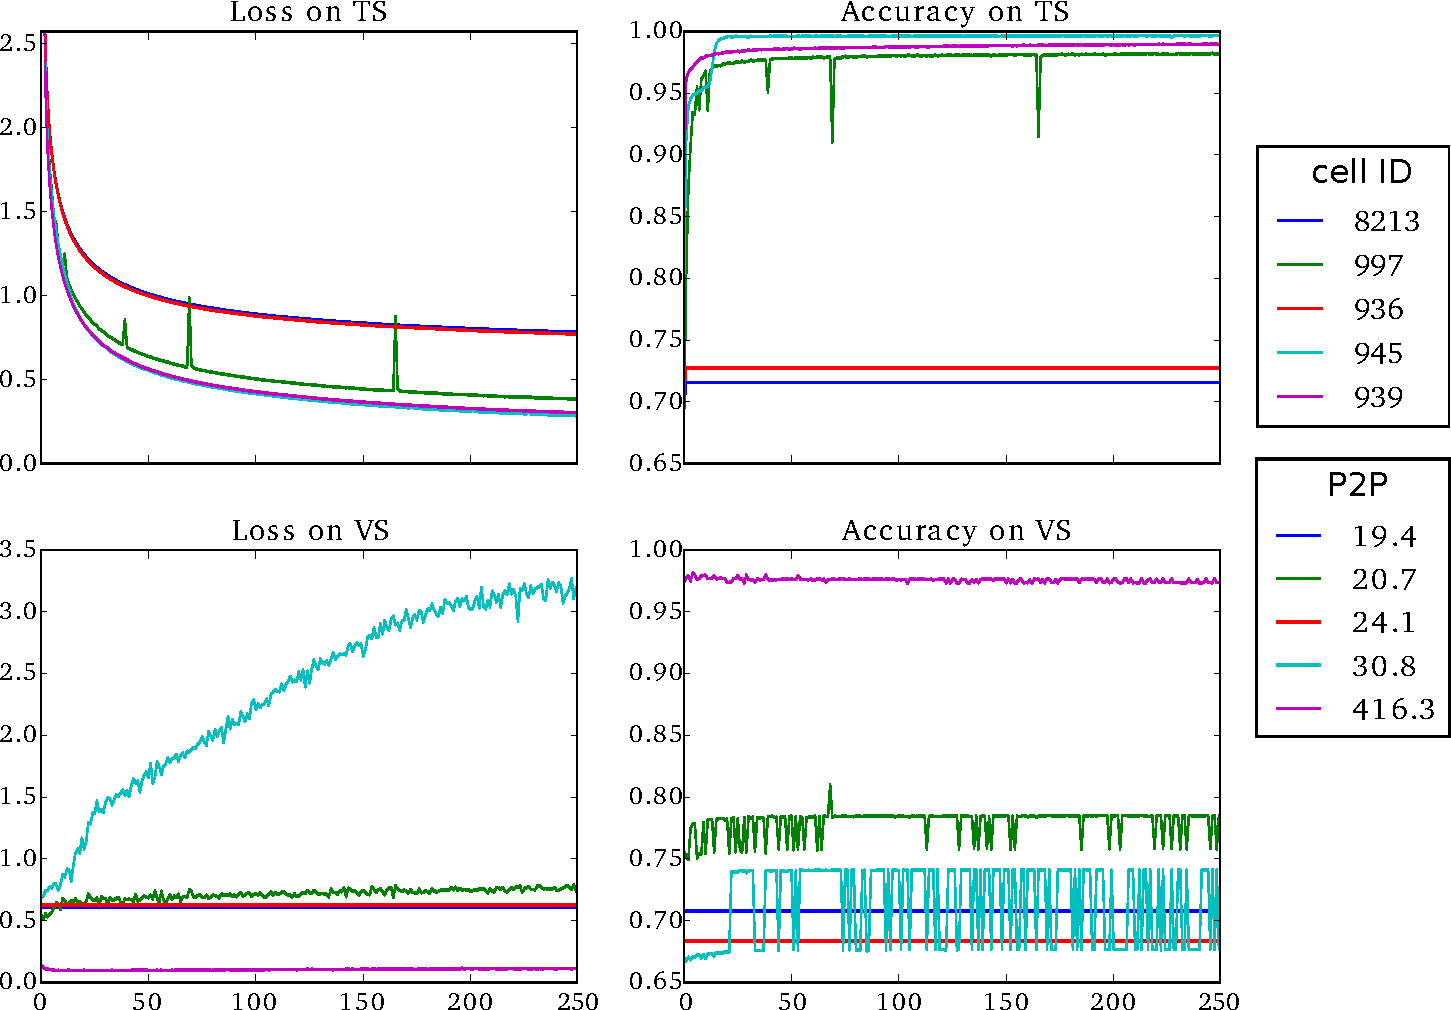
\includegraphics[width=\linewidth]{3.Chapter/study-on-different-cells-norm.pdf}
	\caption{Study on Different Recordings. Loss function and accuracies in the training set and in the validation set.The learning rate was $\eta = 0.01$, the weight decay was fixed at $\lambda = 0.001$, and the initialization method was LeCun Uniform. On the legend on the top is the Cell ID and on the legend on the bottom are the P2P amplitude (in $\mu V$).
}
\label{fig:study-cells}
\end{figure}

The values for the True Positives (TP), True Negatives (TN), False Positives (FP) and False Negatives (FN) at the end of traning were calculated as well as the values for the True Positive Rate (TPR), calculated as :
\begin{equation}
\centering
TPR = \frac{TP}{TP + FN}
\end{equation}

The results are presented in Table \ref{table:confusion-matrix}.

\begin{table}[htb]
\begin{center}
\begin{tabular}{c|cccc|cc}
cell ID & TP & TN & FP & FN & TPR & phy acc.\\ \hline
8213 & 0.00\% & 70.76\% & 0.00\% & 29.24\% & 0.00\% & -0.01\% \\
936 & 0.00\% & 68.35\% & 0.00\% & 31.65\% & 0.00\% & -1.02\% \\ 
939 & 26.85\% & 70.53\% & 0.38\% & 2.24\% & 92.31\% & 46.60\% \\ 
945 & 6.45\% & 67.66\% & 0.07\% & 25.81\% & 20.00\% & 8.38\% \\ 
997 & 2.67\% & 75.80\% & 0.18\% & 21.35\% & 11.11\% & 1.99\% \\ 
\end{tabular}
\end{center}
\caption{Values of the True Positives (TP), True Negatives (TN), False Positives (FP) and False Negatives (FN) at the end of the training, along with the value of the True Positive Rate (TPR). The accuracies achieved with phy in Chapter 2 are also presented. }
\label{table:confusion-matrix}
\end{table}

With the recordings 8213 and 936, the DNN converged to the "zero" solution since the very first epoch and was never able to be "trained out" of the local minimum it got held in. Indeed, in Table \ref{table:confusion-matrix}, the number of false negatives equals the fraction of "1" examples after upsampling (see Table \ref{table:summary-afterUS}).

The recordings 945 and 997 kept oscillating between two "states". In both cases the state with the lowest accuracy corresponds to the "zero" solution, successfully classifying all the "0" labeled examples but failing in the examples labeled as "1". In the other state, the network seems to positively classify 20.0\% and 11.11\% of the "1" examples, respectively.

Trained with the recording from the cell 939, the DNN managed to correctly classify 92.31\% of the EAPs present. 

\section{Discussion}
\label{sec:chap3-discussion}


Looking at Fig. \ref{fig:study-cells} it can be seen that with the chosen training configuration all recordings trained the DNN after only a few epochs: by the epoch 20 the accuracies in all cases reached their final value, or even getting worse afterwards, and therefore applying a stop criteria should be considered.

%%%%%%%%%%%%%%%%%%%%%%   COMPARISON WITH PHY    %%%%%%%%%%%%
Comparing with the results using phy presented in Chapter 2, this method seems to give better results: when the network didn't converge to the "zero" solution, the detection rates more than doubled, reaching a 5-fold increase on the recording 997. However, the detection rates on the recordings 945 and 997 correspond to the detection of only one spike, since the validation set in these case only had 5 and 9 different positive examples. 

It is also important to refer that the oscillations observed with the recording 945 and 997 suggest that the training used work may not be very robust: it appears that the network "jumps" easily between two local minima. Therefore it seems imperative to trained the network with more data. Another possible improvement would be increasing the probability parameter on the dropout procedure.

The recording 939 trained the network into detecting 92.31\%, which is a large value, with very few false positives and false negatives. However, in this recording the P2P amplitude was 416.3 $\mu V$, with a noise standard deviation of 10.51 $\mu V$, and should be easily detected with the conservative application of classic methods such as a threshold-based detection.
%Nonetheless, this method seems to be able to deal with situation of overlapping spikes. 
%As it was discussed in Chapter 2, probably the number of events detected by phy in this recording is underestimated and thus the improvement in this dataset may not be a big as it may seem.

In reality, the configurations and hyperparameters considered optimal were only studied with the recording 939 and may not be optimal for all datasets.

It should be noted that it is very likely that the windows labeled as "0" have many other spikes. This may actually make the training process much more difficult: since the production of any EAP relies on similar physical process, many spikes may be very similar to the spike from the juxta neuron, making the distinction, and thus the training, more difficult. For this reason, using a bigger dataset should return significantly better results, in particular, a bigger dataset with more different positive examples. The upsampling step may have forced the training to give a larger importance to each positive example but it didn't feed the network any new information about the event of interest. Possibly it could have been better to, instead of upsampling, perform downsampling or both: reduce the number of negative examples and increase the number of positive examples. In this way, more variability on the positive examples would be taken into consideration, making the network learn the useful structure of the EAPs better.

In the recording 8213 there were 202 different positive examples in the training set, more or less the same as in recording 939 which had 207. Nonetheless, the DNN was trained into the "zero" solution. At the same time this recording was the lowest in amplitude, with a $19.4 \mu V$ P2P amplitude, and the one with the highest noise standard deviation of $12.95 \mu V$, therefore most of the example are probably "drowned" in the noise, preventing the DNN to see the signal of interest. This suggests that there may be a threshold SNR below which this method cannot be applied, perhaps regardless of how many spikes there are in the training set.

It is important to keep in mind the question we're training the network to answer: whether or not, in a certain time window, there was a spike from this particular cell, and not a spike from any cell. Indeed, each network was trained with only one dataset individually. It would be interesting to train a DNN with different datasets recorded with the same probe. In this situation the question would be different: in this time window is a there a spike from this set of targeted cells? This would not only increase the number of examples (in particular positive examples), but also make this procedure more generalizable and applicable in more situations when enough different datasets have been used. However, this would affect the training: it may make it easier if the datasets are similar, or it may make it harder if there is a big difference in  EAPs from the considered juxta neurons. 

It is never too much noting that this new dataset would have to shuffled if the training algorithm doesn't do it for us, for instance if we train the network in chunks of data due to memory contraints. Otherwise, on the first epochs of training the DNN would "crystalize" on detecting that particular first EAP and may be harder to train it away from that configuration to learn the new EAPs. 
Another way to achieve this would be producing a hybrid dataset where many ground truth datasets are brought together, for examples as an average or hand-crafted, to produce one simulated recording with larger variability on the positive examples without increasing the size of the dataset, and therefore improving the unbalance in the dataset.

As mentioned above, due to memory the time windows were time shifted from the previous by 5 samples. Windows whose central sample were closest to each time juxta time where labeled as positives. Therefore if sequential time windows were presented, the DNN would probably yield 5  positive predictions per juxta spike.
\cleardoublepage

% %%%%%%%%%%%%%%%%%%%%%%%%%%%%%%%%%%%%%%%%%%%%%%%%%%%%%%%%%%%%%%%%%%%%%%
% The Introduction:
% %%%%%%%%%%%%%%%%%%%%%%%%%%%%%%%%%%%%%%%%%%%%%%%%%%%%%%%%%%%%%%%%%%%%%%
\fancychapter{Conclusions and Future Work}
\label{cap:conclusions}

\section{Future Directions}
In this work, I tried to assess the viability of the pursuit of better spike detection algorithms in the context of deep learning. I tried to implement feed-forward deep neural networks to detect Extracellular Action Potential of one particular neuron in each training of the DNN. Comparing it with the state-of-the-art algorithm designed to detect these spikes (phy) seems to lead the conclusion such pursuit is worthy, since the deep learning approach yielded better results. This work should, however, be regarded as a "proof of concept". Indeed, much remains to be done. In the particular framework of this document, the architecture, configuration and hyperparameters should be further studied to provide as universally optimal values as possible for learning with any dataset.

The datasets I based this work on were recorded using 127-channel planar probe spanning over 90 $\mu m$ in one direction and 717.5 $\mu m$ on the other. Neurons in its vicinity usually only impress a small portion of the probe. Therefore a spike detection algorithm for such probe should be agnostic to where the neuron's footprint rests. In other words, it should translation invariant. So, moving away from this work, I think it should be useful to try applying Convolutional Neural Networks, where the adjustable parameters are actually many small sized kernels that shall be convoluted with the output of the previous layer. Regardless of where the neuron's footprint appeared a well-trained kernel  would be run through the whole probe and would eventually result in a positive identification.

The success in identifying the spikes in the 

Another possible use for deep neural network would be to train a noise filter. The raw filtered signal would be fed in the input layer and then supervised learning would train the DNN to provide the Juxta-Triggered Averages (JTA). If successfully trained, the resulting output would be relatively noise-free and a simple threshold-based detection algorithm could be applied. If many different recordings were utilized, perhaps the resulting DNN could be universal and used in any recording. Analysing the layers of this trained network, this could also help researchers understand what the biological noise in the extracellular medium really is.

\cleardoublepage

\cleardoublepage
\phantomsection
\addcontentsline{toc}{chapter}{Bibliography}
\bibliographystyle{plain}
\bibliography{02.biblio}
\cleardoublepage

\begin{appendices}
	\begin{appendix}
		\pagenumbering{bychapter}
		\fancychapter{Cross-Correlograms per electrode}
\label{ap:a}

\begin{landscape}
%, width=\linewidth
\begin{figure}[!h]
	\centering
	\includegraphics[height=\textheight]{Ap1/CC-per-channel.pdf}
	\caption{Cross-Correlograms between the juxta spikes and the phy-detected events on each electrode. On the left is the bottom half of the probe and on the right top half of the probe. The size of the bins in the histograms is 1 ms and the value for the lag is 50ms.
}
\label{fig:CC-per-channel}
\end{figure}

\end{landscape}   
		\cleardoublepage
	\end{appendix}
\end{appendices}


\end{document}
